% 2018. 06. 11. DLC LaTeX Lecture
\documentclass[10pt, mathserif, aspectratio=169]{beamer}


%---------------------------------------------------------------
% INCLUDE PACKAGES
%---------------------------------------------------------------
\usepackage[utf8]{inputenc}
%\usepackage[english]{babel}
%\usepackage[T1]{fontenc}
%\usepackage{helvet}
\usepackage{kotex}
\usepackage{amsmath, amssymb, amsthm, latexsym}
\usepackage{array, booktabs, tabularx}
\usepackage{xcolor}
\usepackage{listings}
%\usepackage{xetexko}



%---------------------------------------------------------------
% USE THEME
%---------------------------------------------------------------
\usetheme{CambridgeUS}

\useinnertheme{rounded}

\usecolortheme{lily}


%---------------------------------------------------------------
% SET HANGUL FONTS
%---------------------------------------------------------------
%\setmainhangulfont{}
%\setsanshangulfont{}
%\setmonohangulfont{}


%---------------------------------------------------------------
% DEFINE USEFUL COLORS
%---------------------------------------------------------------
\definecolor{BoxCol}{rgb}{0.58, 0.05, 0.3}
\definecolor{SectionCol}{rgb}{1, 1, 1}
\definecolor{TextColR}{rgb}{0.9, 0, 0}
\definecolor{TextColG}{rgb}{0, 0.7, 0}
\definecolor{TextColB}{rgb}{0, 0, 0.8}
\newcommand{\Rcolor}{\textcolor{TextColR}}
\newcommand{\Gcolor}{\textcolor{TextColG}}
\newcommand{\Bcolor}{\textcolor{TextColB}}


%---------------------------------------------------------------
% MISCELLANEOUS DEFINITION
%---------------------------------------------------------------
\makeatletter
\def\verbatim@font{\scriptsize\ttfamily}
\makeatother




%---------------------------------------------------------------
% INFORMATION IN THE TITLE PAGE
%---------------------------------------------------------------
\title[\LaTeX{} Lecture]
{ % is placed on the title page
    \LARGE
    \textbf{\LaTeX{} Lecture}
}
    
    
%\subtitle[]
%{ % is placed on the subtitle page
%    \small
%    \textit{\\Nicolas Ballas, Li Yao, Chris Pal, Aaron Courville\\
%        \href{https://arxiv.org/abs/1511.06432}{arXiv: 1511.06432}}
%}
 

\author[Il Gu Yi]
{
    Il \ Gu \ Yi
}


\institute[]
{
  DLC \LaTeX{} Lecture
}

\date{\today}



\logo{
\includegraphics[height=0.7cm]{figures/modu}}




%---------------------------------------------------------------
% THE BODY OF THE PRESENTATION
%---------------------------------------------------------------

\begin{document}


%---------------------------------------------------------------
% THE TITLE PAGE
%---------------------------------------------------------------
%\begin{frame}[plain,noframenumbering]
\begin{frame}
    \titlepage
\end{frame}


\begin{frame}{Content}{}
\tableofcontents
\end{frame}




%---------------------------------------------------------------
\section{알아두어야 할 기본 사항}
%---------------------------------------------------------------
\begin{frame}{오늘 자료는}
%---------------------------------------------------------------
\begin{itemize}
  \item \LaTeX의 가장 유명한 document: The Not So Short Introduction to \LaTeXe (\emph{Or \LaTeXe in 141 minutes})의 한글판
  \item \LaTeXe 입문 ({142분 동안 익히는 \LaTeXe}) - (왜 번역하면서 1분이 늘었났는지는 모르겠음)
  \item (제가 만든) 슬라이드 요약본 입니다. (사실상 ctrl+c, ctrl+v 입니다.)
    \pause
  \item 따라서 142분 보다 짧게 해야 의미가 있을거 같아요.
  \item 안 그러면 여러분들이 그냥 문서를 읽는거랑 같으니까요.
  \item 그래도 결국 \LaTeX을 쓰시려면 저 문서를 한번씩은 보실겁니다.
\end{itemize}
\end{frame}


%---------------------------------------------------------------
\begin{frame}{어떻게 불러야 하는가}
%---------------------------------------------------------------
\begin{itemize}
  \item \LaTeX은 Donald E. Knuth가 만든 컴퓨터 프로그램이다.
  \item \LaTeX은 텍스트와 수학식을 조판하기 위해 만들어졌다.
  \item \LaTeX은 "tech"로 발음한다\footnote{\LaTeX 2$\epsilon$ 입문}.
  \item \LaTeX (LAH-tekh or LAY-tekh; a shortening of Lamport TeX) is a document preparation system\footnote{wikipedia}.
\end{itemize}
\end{frame}


%---------------------------------------------------------------
\begin{frame}{기본 사항}
%---------------------------------------------------------------
\begin{block}{저자, 디자이너, 조판사}
  \begin{enumerate}
    \item 책을 출판할 때 저자는 타자기로 원고를 작성하여 출판사에 넘겨준다.
    \item 그 회사의 북디자이너 한 명이 이 문서의 레이아웃(외양: 문단폭, 글꼴, 제목줄 앞 뒤의 여백 ...)을 결정한다.
    \item 디자이너는 자신의 지시사항을 원고에 써 넣은 다음 조판사에게 넘긴다.
    \item 조판사는 이 지시사항에 따라 책을 조판한다.
  \end{enumerate}
\end{block}

\pause
\vspace{0.5ex}

\begin{block}{\center 그럼 \LaTeX의 역할은?}
\pause
\center \LaTeX은 Designer
\end{block}

\pause
\vspace{0.5ex}

\begin{block}{}
  \begin{itemize}
    \item 그러나 LATEX은 단지 컴퓨터 프로그램에 지나지 않습니다.
    \item 따라서 사람 인 디자이너에게 맡기는 경우보다 더 많은 지시사항을 알려주어야 할 것이다.
    \item 이것이 {\bf \LaTeX{} 명령} 또는 {\bf \LaTeX{} 문법}을 배워야 하는 이유입니다.
  \end{itemize}
\end{block}

\end{frame}


%---------------------------------------------------------------
\begin{frame}{레이아웃 디자인}
%---------------------------------------------------------------
\begin{block}{WYSIWYG (What you see is what you get)}
\begin{itemize}
  \item MS Word나 한글따위와는 질적으로 다르다.
  \item *.tex 파일에 문법에 맞게 글을 쓰고 이를 \LaTeX으로 컴파일(?)해야 출력결과를 볼 수 있다.
  \item WYSIWYG 시스템을 사용하는 저자들은 외관상 보기에는 좋을지 몰라도 도대체 구조적이지 못하고 일관성도 없는 문서를 만들어내는 경우가 많다.
  \begin{itemize}
    \item 한글을 쓰면서 1. Introduction 1.1 Machine Learning 쓰면서 서로 다른 글꼴 선언하기 위해 얼마나 개고생을 했던가.
    \item 서식을 맞추기 위해 서식복사 alt+c 를 했었지.
  \end{itemize}
  \item \LaTeX은 저자 자신의 문서에 {\bf 논리적인 구조}를 선언하게 함으로써 이러한 구조 오류를 피하게 해준다.
\end{itemize}
\end{block}
\end{frame}


%---------------------------------------------------------------
\begin{frame}{장점과 단점 (1)}
%---------------------------------------------------------------
\begin{block}{장점}
\begin{itemize}
  \item 전문가 수준으로 디자인된 레이아웃을 사용할 수 있다. 그래서 문서가 “인쇄된” 것과 거의 동일하다.
  \item 수학식의 조판이 매우 쉽다.
  \begin{itemize}
    \item 한글도 수식의 조판이 쉽다. 왜냐하면 \LaTeX{} 수식 문법을 거의 그대로 배꼈기 때문이다.
  \end{itemize}
  \item 사용자는 문서의 논리적 구조를 지시하는 몇 가지 기억하기 쉬운 명령어들만 익히면 된다.
  \item 각주, 상호참조, 목차, 참고문헌 등 매우 복잡한 구조들도 아주 쉽게 만들어진다.
  \item \LaTeX{} 기본 패키지 이외에도 여러 가지 조판상의 필요를 충족시키는 자 유롭게 이용할 수 있는 추가 패키지들이 많다.
  \item \LaTeX은 구조화가 잘된 문서를 작성하도록 저자를 유도한다. \LaTeX의 동작 방식이 바로 그것이다({\bf 구조를 지정}하는 것).
  \item \LaTeX2e의 조판 엔진인 \LaTeX은 매우 이식성이 높으며 free software이다.
\end{itemize}
\end{block}
\end{frame}


%---------------------------------------------------------------
\begin{frame}{장점과 단점 (2)}
%---------------------------------------------------------------
\begin{block}{단점 (없지만 굳이 쓰자면)}
  \pause
  \begin{itemize}
    \item \LaTeX은 아무 생각 없는 머리가 빈 사람들하고는 잘 맞지 않는다.
    \item 미리 만들어진 레이아웃 인자의 기정값을 조절해가면서 쓸 수 있기는 하지만, 완전히 새로운 레이아웃을 설계하는 것은 어렵고 시간이 많이 드는 일이다.
    \item 구조화되지 않고 비체계적인 문서를 작성하기가 너무나 어렵다.
    \item 햄스터에게는 아무리 노력해도 논리적 마크업의 개념을 이해시키기 쉽지 않을 것이다.
  \end{itemize}
\end{block}
\end{frame}


%---------------------------------------------------------------
\begin{frame}{\LaTeX{} 컴파일}
%---------------------------------------------------------------
\begin{block}{\LaTeX{} 작업순서}
  \begin{enumerate}
    \item \LaTeX{} 파일(.tex)을 만든다.
    \begin{itemize}
      \item 이 파일은 플레인 텍스트 파일 이어야 한다.
      \item 유닉스 시스템의 모든 에디터는 플레인 텍스트 파일을 만든다.
      \item 윈도우에서라면 파일을 ASCII 또는 plain text 포맷으로 저장해야 할 것이다.
      \item 파일 이름은 확장명을 {\sf .tex}으로 붙인다.
    \end{itemize}
    \item {\sf pdflatex} 명령어로 컴파일을 한다. ({\sf pdflatex foo.tex})
    \begin{itemize}
      \item 목차나 내부 상호참조를 완성하려면 {\sf pdflatex}을 두세번 실행해야 할 것이다.
    \end{itemize}
  \end{enumerate}
\end{block}
\end{frame}


%---------------------------------------------------------------
\begin{frame}[fragile]{\LaTeX{} 입력 파일의 구조 (1)}
%---------------------------------------------------------------
\begin{block}{필수요소}
  \begin{itemize}
    \item {\sf \textbackslash documentclass\{...\}} 
    \begin{itemize}
      \item 이 명령은 지금 작성하고자 하는 문서가 어떤 종류의 것인지 설정하는 것이다.
    \end{itemize}
    \item {\sf \textbackslash usepackage\{...\}} 
    \begin{itemize}
      \item 전체 문서의 모양(스타일)에 영향을 주는 명령들을 포함하거나 \LaTeX{} 시스템에 새로운 기능을 추가하는 패키지들을 포함할 때 쓴다.
    \end{itemize}
    \item {\sf \textbackslash begin\{...\}} 
    \item {\sf \textbackslash end\{...\}} 
  \end{itemize}
\end{block}

\begin{block}{가장 간단한 \LaTeX{} 파일을 만들어보자 (example01.tex)}
\begin{lstlisting}
\documentclass{article}
\begin{document}
Hello, \LaTeX.
\end{document}
\end{lstlisting}
\end{block}

\end{frame}


%---------------------------------------------------------------
\begin{frame}[fragile]{\LaTeX{} 입력 파일의 구조 (2)}
%---------------------------------------------------------------
\begin{block}{실제 학술지 논문의 보기 (example02.tex)}
{\scriptsize
\begin{lstlisting}
\documentclass[a4paper,11pt]{article}

% define the title
\author{H.~Partl}
\title{Minimalism}

\begin{document}
% generates the title
\maketitle

% insert the table of contents
\tableofcontents

\section{Some Interesting Words}
Well, and here begins my lovely article.

\section{Good Bye World}
\ldots{} and here it ends.

\end{document}
\end{lstlisting}}
\end{block}
\end{frame}


%---------------------------------------------------------------
\begin{frame}{\LaTeX{} 실제 입력 방식 (1)}
%---------------------------------------------------------------
\begin{block}{공백}
\begin{itemize}
  \item "공백문자(whitespace characters)", 즉 빈 칸(blank), 탭(tab) 등은 \LaTeX에서 모두 동일하게 "스페이스"로 처리된다.
  \item 계속되는 여러개의 공백문자들은 하나의 "스페이스"로 취급된다.
  \item 행의 첫머리에 있는 공백문자들은 무시되고 한 번의 줄바꿈(개행:linebreak) 역시 "공백문자"로 간주된다.
  \item 두 줄 사이에 빈 줄을 하나 넣으면 문단(paragraph)의 끝을 나타낸다.
  \item 빈 줄을 여러개 넣어도 한줄을 넣은 것과 효과가 같다. 
\end{itemize}
\end{block}

\begin{figure}
  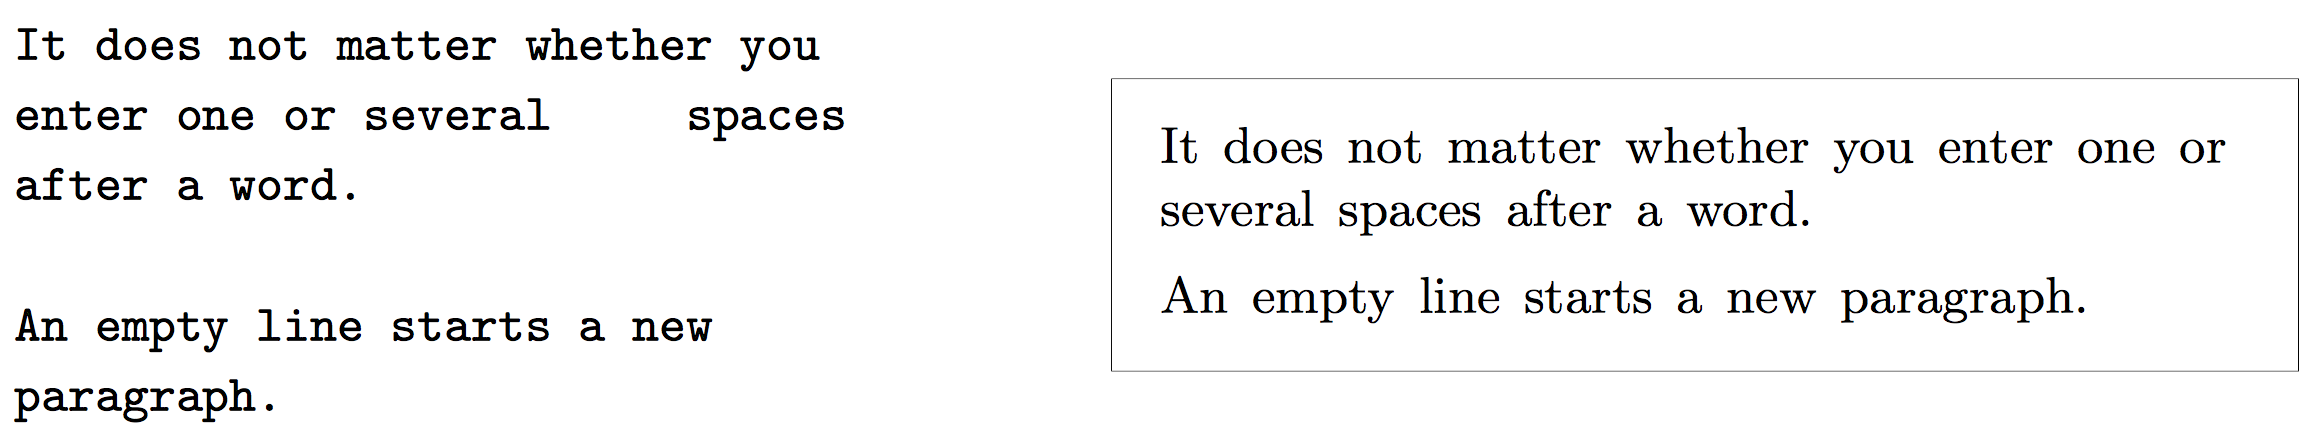
\includegraphics[width=0.7\textwidth]{figures/1_3_1_whitespace}
\end{figure}

\end{frame}

%---------------------------------------------------------------
\begin{frame}{\LaTeX{} 실제 입력 방식 (2)}
%---------------------------------------------------------------
\begin{block}{특수문자}
\begin{itemize}
  \item \# \$ \% \^{} \& \_ \{ \} \~{} 이런 특수문자를 쓰려면
\end{itemize}
\end{block}

\begin{figure}
  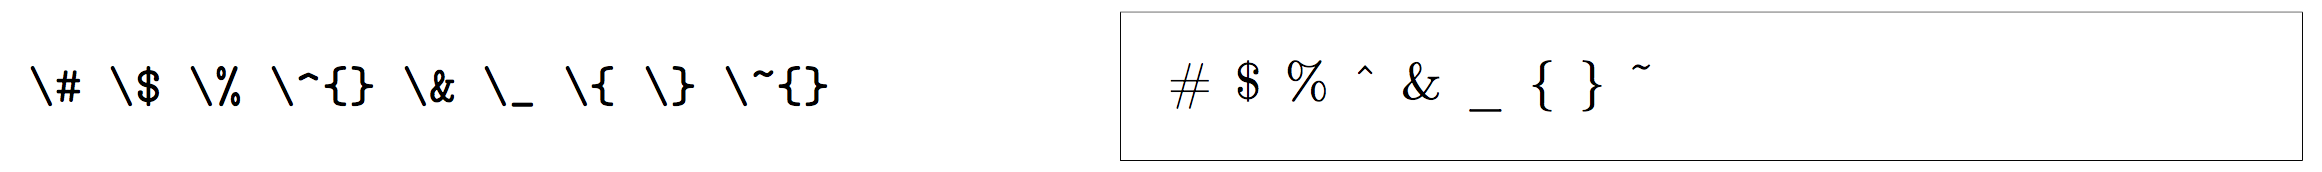
\includegraphics[width=0.7\textwidth]{figures/1_3_2_special_character}
\end{figure}

  \pause
\begin{block}{그럼 \textbackslash는 어떻게 입력하지?}
  \pause
\begin{itemize}
  \item \textbackslash textbackslash
\end{itemize}
\end{block}

\end{frame}


%---------------------------------------------------------------
\begin{frame}{\LaTeX{} 실제 입력 방식 (3)}
%---------------------------------------------------------------
\begin{block}{\LaTeX{} 명령}
\begin{itemize}
  \item 백슬래시 \textbackslash 로 시작하여 문자(letter)만으로 이루어진 이름을 갖는다.
  \item 명령 이름은 공백이나 숫자 또는 '문자 아닌 것'이 오면 끝난다.
  \item 백슬래시 다음에 딱 한 개의 기타 문자(non-letter)가 온다.
  \item \LaTeX은 명령 다음의 공백문자를 무시한다.
  \item 명령 다음에 빈 칸을 두고 싶으면 \{\}와 빈 칸을 써넣거나 명령 이름 뒤에 특별한 칸 띄우기 명령을 써야 한다.
\end{itemize}
\end{block}

\begin{figure}
  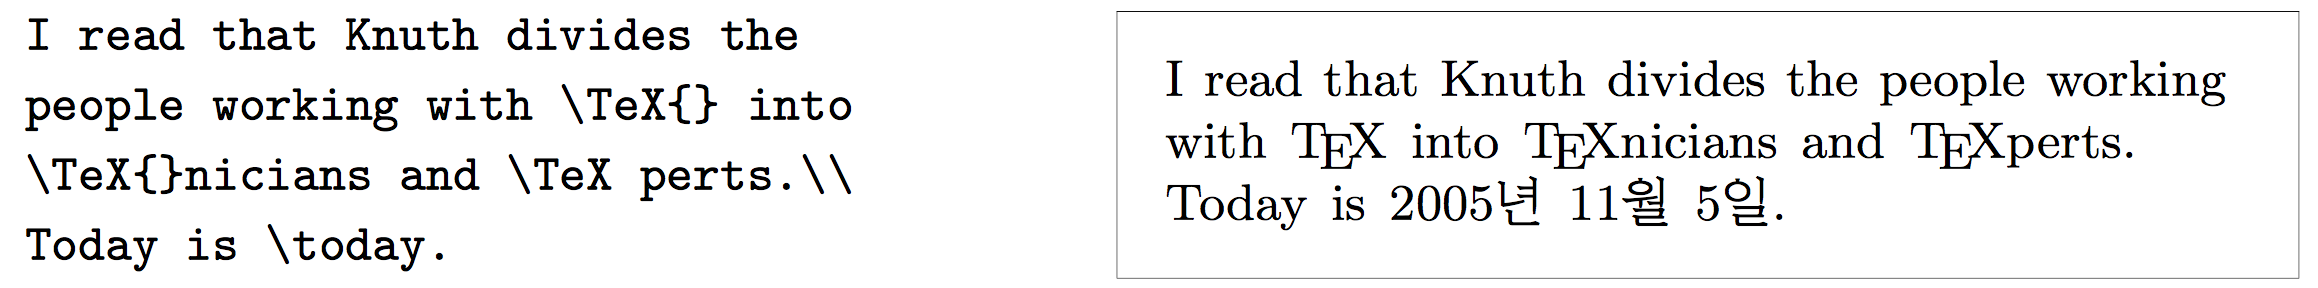
\includegraphics[width=0.7\textwidth]{figures/1_3_3_latex_command1}
\end{figure}
\end{frame}


%---------------------------------------------------------------
\begin{frame}{\LaTeX{} 실제 입력 방식 (4)}
%---------------------------------------------------------------
\begin{block}{}
\begin{itemize}
  \item 인자(parameter)가 필요한 명령도 있다.
  \item 인자는 명령 이름 다음의 중괄호 \{ \} 속에 써넣어야 한다.
  \item 어떤 명령에는 옵션 인자(optional parameters)가 필요한 경우도 있는데, 명령 바로 다음에 대괄호 [ ]를 쓰고 그 안에 써넣는다.
\end{itemize}
\end{block}

\begin{figure}
  
\includegraphics[width=0.7\textwidth]{figures/1_3_3_latex_command2}
\end{figure}
\begin{figure}
  
\includegraphics[width=0.7\textwidth]{figures/1_3_3_latex_command3}
\end{figure}
\end{frame}


%---------------------------------------------------------------
\begin{frame}{\LaTeX{} 실제 입력 방식 (5)}
%---------------------------------------------------------------
\begin{block}{주석}
\begin{itemize}
  \item \%문자를 쓴다.
  \item \%문자는 공백문자나 줄바꿈 문자가 허용되지 않는 긴 줄을 나누어 입력할 수 있게 해준다.
\end{itemize}
\end{block}
\begin{figure}
  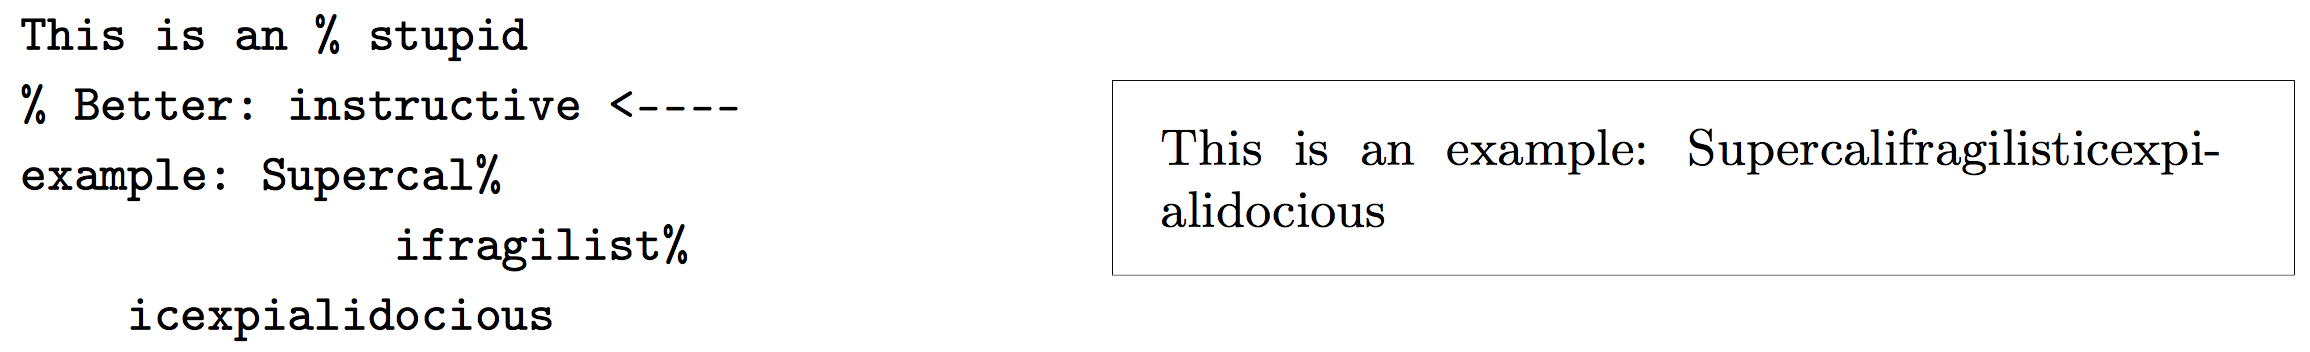
\includegraphics[width=0.7\textwidth]{figures/1_3_4_comments}
\end{figure}

\end{frame}


%---------------------------------------------------------------
\begin{frame}{레이아웃}{문서 클래스 (1)}
%---------------------------------------------------------------
{\sf \textbackslash documentclass[options]\{class\}}
\begin{block}{{\sf class} 인자}
\begin{description}
  \item[article] 과학 학술지, 프리젠테이션, 짧은 보고서, 프로그램 문서, 초대장 등에 쓰이는 아티클용 클래스
  \item[proc] article 클래스에 기초한 프로시딩을 위한 클래스
  \item[minimal] 최소 문서 양식 클래스. 페이지 크기와 기본 글꼴만을 설정한다. 주로 디버깅을 위하여 사용
  \item[report] 여러 장(chapter)으로 이루어진 긴 보고서, 작은 책, 박사학위 논문 등에 쓰이는 클래스
  \item[book] 진짜 책을 만들기 위한 클래스
  \item[beamer] 슬라이드 제작용 클래스
\end{description}
\end{block}
\end{frame}


%---------------------------------------------------------------
\begin{frame}{레이아웃}{문서 클래스 (2)}
%---------------------------------------------------------------
{\sf \textbackslash documentclass[options]\{class\}}
\begin{block}{{\sf options} 인자}
\begin{description}
  \item[10pt, 11pt, 12pt] 문서 기본 글꼴 크기를 설정. default option: 10pt
  \item[a4paper, letterpaper, ...] 종이 크기를 지정. default option: letterpaper. others: a5paper, b5paper, executivepaper, legalpaper.
  \item[onecolumn, twocolumn] 문서를 1단 또는 2단으로 조판하도록 지시
  \item[landscape] 레이아웃을 가로가 긴 형식(landscape)으로 변경.
\end{description}
\end{block}
\end{frame}


%---------------------------------------------------------------
\begin{frame}[fragile]{레이아웃}{패키지}
%---------------------------------------------------------------
{\sf \textbackslash usepackage[options]\{package\}}
\begin{block}{for example (지금 이 beamer에 사용된 packages)}
\begin{lstlisting}
\usepackage[utf8]{inputenc}
\usepackage{kotex}
\usepackage{amsmath, amssymb, amsthm, latexsym}
\usepackage{array, booktabs, tabularx}
\usepackage{xcolor}
\usepackage{listings}
\end{lstlisting}
\end{block}
\end{frame}


%---------------------------------------------------------------
\begin{frame}{작업 과정에 생성되는 파일들}
%---------------------------------------------------------------
\begin{block}{{\sf latex} 으로 컴파일할 때 생성되는 파일들}
\begin{description}
  \item[.dvi] 장치 독립(device independent) 파일. \LaTeX의 주 출력 형식이다.
  \item[.log] 직전의 컴파일 과정에서 무슨 일이 일어난 것인지를 상세하게 알려주는 로그 파일.
  \item[.toc] 장절 표제를 저장해 두는 파일. 다음 번 컴파일 때 \LaTeX이 읽어서 목차를 만드는 데 사용한다.
  \item[.lof] .toc와 같지만 그림 목차에 해당한다.
  \item[.lot] 표 목차를 위한 파일이다.
  \item[.aux] 컴파일러는 필요한 정보를 이 파일에 적어서 다음 번 실행때 읽어들이도록 한다. 주로 상호참조를 완성하기 위해 쓰인다.
\end{description}
\end{block}
\end{frame}




%---------------------------------------------------------------
\section{텍스트의 조판}
%---------------------------------------------------------------
\begin{frame}{줄바꿈과 쪽나눔}
%---------------------------------------------------------------
  \begin{block}{단락 정렬 (example03.tex)}
\begin{description}
  \item[\textbackslash\textbackslash{} 또는 \textbackslash newline] 다음 명령은 새 단락을 시작하지 않으면서 줄을 바꾼다.
  \item[\textbackslash\textbackslash *] 다음 명령은 강제로 줄을 바꾸면서 쪽나눔은 일어나지 않도록 한다.
  \item[\textbackslash newpage] 새 쪽을 시작하려면 다음 명령을 이용한다.
\end{description}
\end{block}
\end{frame}


%---------------------------------------------------------------
\begin{frame}{미리 정의된 문자열}
%---------------------------------------------------------------
\begin{block}{특별한 문자열}
  \center
\begin{tabular}{lll}
명령어 & 사용예 & 설명 \\
\hline
\textbackslash today & 2018년 6월 14일 & 현재 사용 언어에서의 현재 날짜 표기 \\
\textbackslash LaTeX & \LaTeX & 지금 우리가 배우고 있는 것의 이름 \\
\textbackslash LaTeXe & \LaTeXe & LATEX의 최신판 \\
\end{tabular}
\end{block}
\end{frame}
%---------------------------------------------------------------
\begin{frame}{특수 문자와 기호}
%---------------------------------------------------------------
\begin{block}{대시와 하이픈}
\begin{figure}
  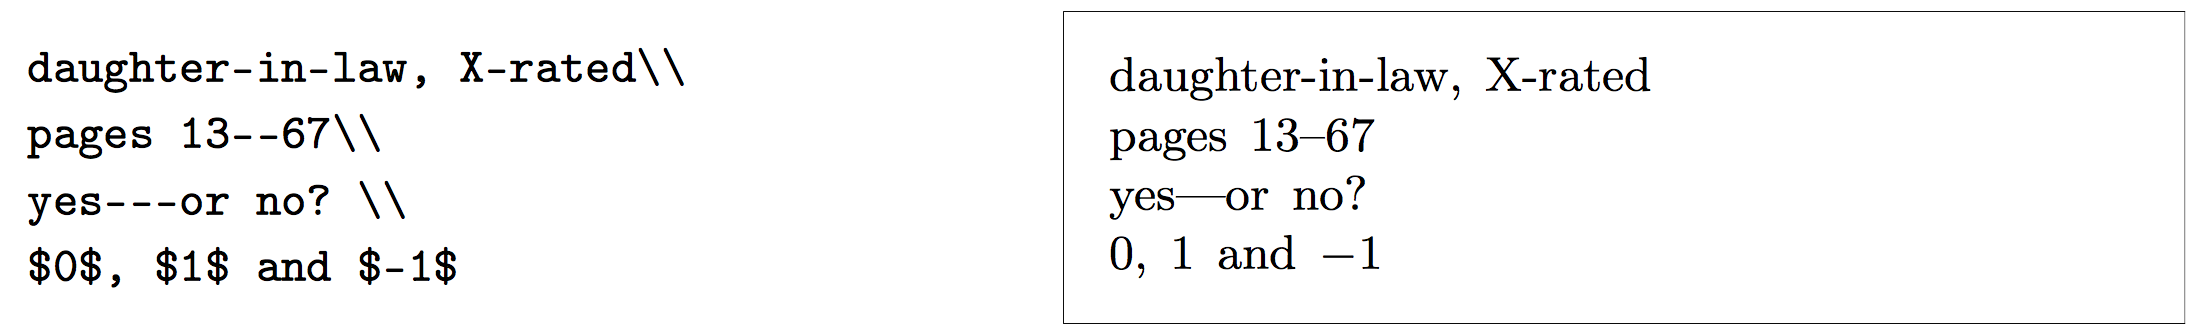
\includegraphics[width=0.7\textwidth]{figures/2_4_2_dash}
\end{figure}
이 대시들은 각각 '-' 하이픈, '--' 엔대시, '---' 엠대시 그리고 '$-$' 빼기 부호 라고 한다.
\end{block}

  \pause
  \begin{block}{틸데(\~{})}
\begin{figure}
  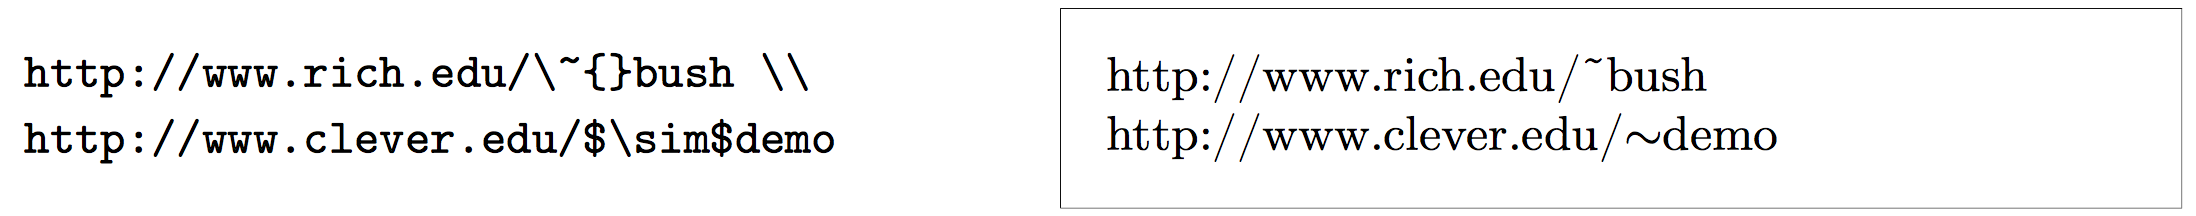
\includegraphics[width=0.7\textwidth]{figures/2_4_3_tilde}
\end{figure}
\end{block}
\end{frame}


%---------------------------------------------------------------
\begin{frame}{강세 부호와 특수 문자}
%---------------------------------------------------------------
\begin{block}{대시와 하이픈}
\begin{figure}
  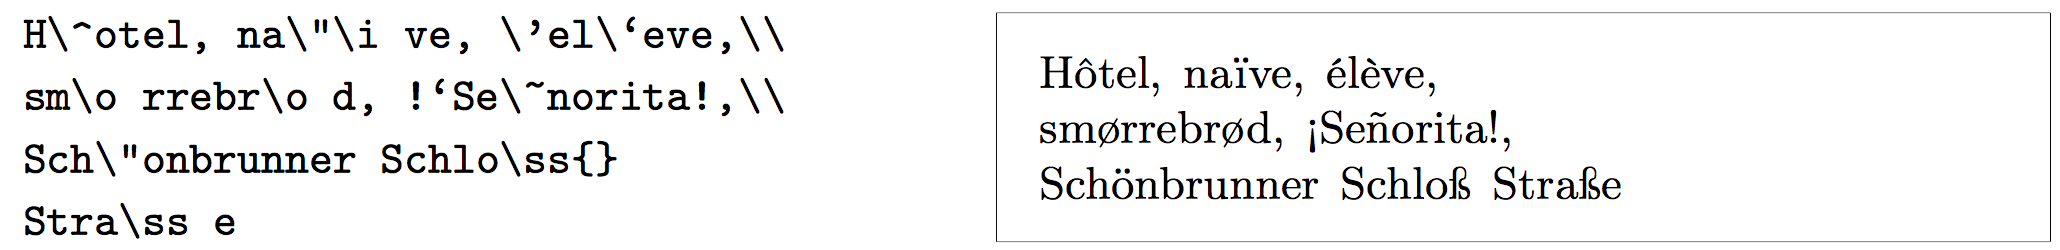
\includegraphics[width=0.7\textwidth]{figures/2_4_8_accent_characters1}\\
    \vspace{1ex}
  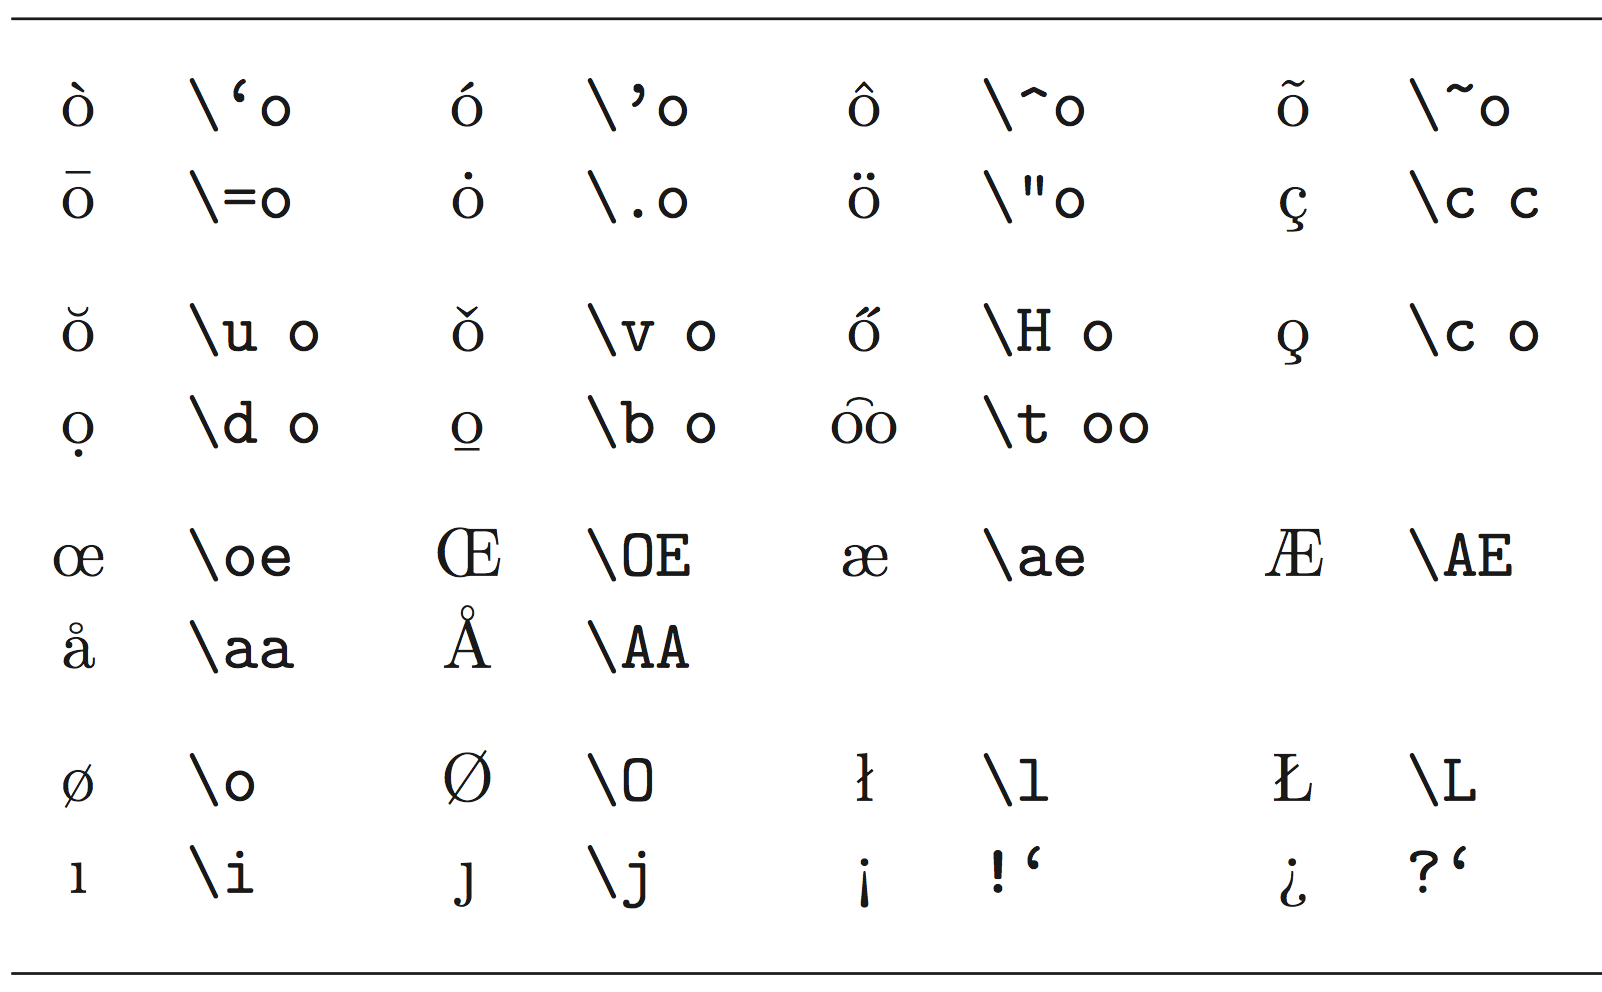
\includegraphics[width=0.45\textwidth]{figures/2_4_8_accent_characters2}
\end{figure}
\end{block}
\end{frame}


%---------------------------------------------------------------
\begin{frame}{제목과 장 절}{(example04.tex)}
%---------------------------------------------------------------
\begin{block}{structure of article class}
\begin{itemize}
  \item \textbackslash section\{...\}
  \item \textbackslash subsection\{...\}
  \item \textbackslash subsubsection\{...\}
  \item \textbackslash paragraph\{...\}
  \item \textbackslash subparagraph\{...\}
\end{itemize}
\end{block}

\begin{block}{structure of report and book classes}
\begin{itemize}
  \item \textbackslash part\{...\}
  \item \textbackslash chapter\{...\}
\end{itemize}
\end{block}
\end{frame}


%---------------------------------------------------------------
\begin{frame}{상호참조}{(example05.tex)}
%---------------------------------------------------------------
\begin{block}{}
\begin{itemize}
  \item \textbackslash label\{\emph{marker}\}
  \item \textbackslash ref\{\emph{marker}\}
  \item \textbackslash pageref\{\emph{marker}\}
\end{itemize}
\end{block}

\begin{figure}
  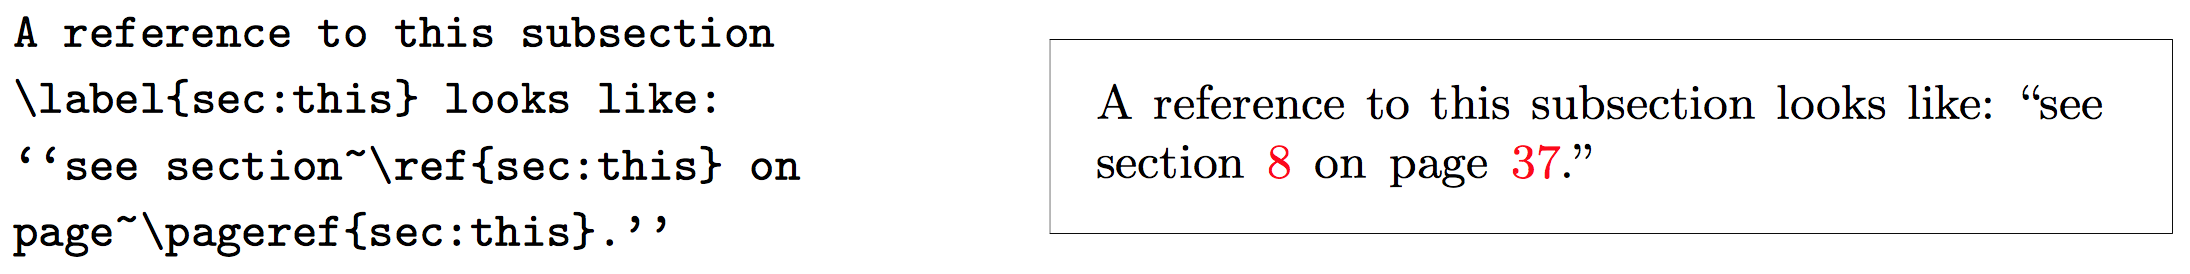
\includegraphics[width=0.7\textwidth]{figures/2_8_ref}
\end{figure}

\end{frame}


%---------------------------------------------------------------
\begin{frame}{각주}
%---------------------------------------------------------------
\begin{block}{}
\begin{itemize}
  \item \textbackslash footnote\{\emph{footnote text}\}
\end{itemize}
\end{block}

\begin{figure}
  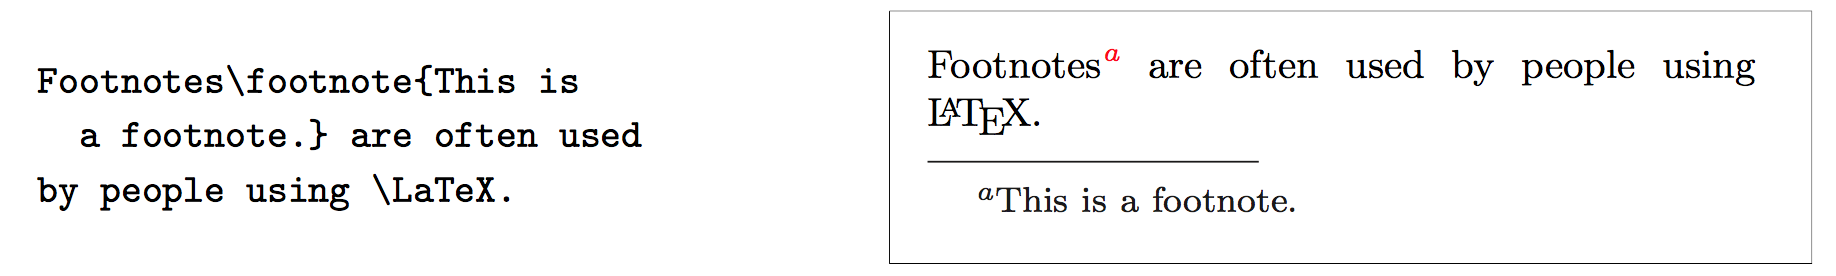
\includegraphics[width=0.7\textwidth]{figures/2_9_footnote}
\end{figure}
\end{frame}


%---------------------------------------------------------------
\begin{frame}{강조}
%---------------------------------------------------------------
\begin{block}{}
\begin{itemize}
  \item \textbackslash underline\{\emph{text}\}
  \item \textbackslash emph\{\emph{text}\}
\end{itemize}
\end{block}

이 명령의 실제 동작은 앞뒤 문맥에 따라 다르다.
\begin{figure}
  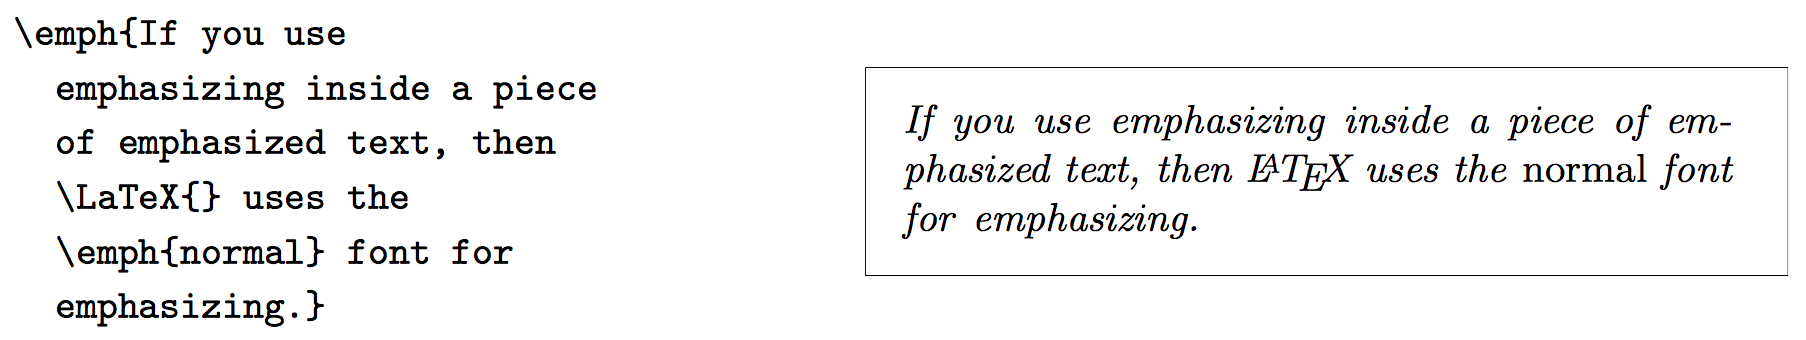
\includegraphics[width=0.6\textwidth]{figures/2_10_emph1}
\end{figure}

\LaTeX에게 무엇인가를 {\bf 강조}하게 하는 것과 다른 {\bf 글꼴}을 사용하게 하는 것은 다르다.
\begin{figure}
  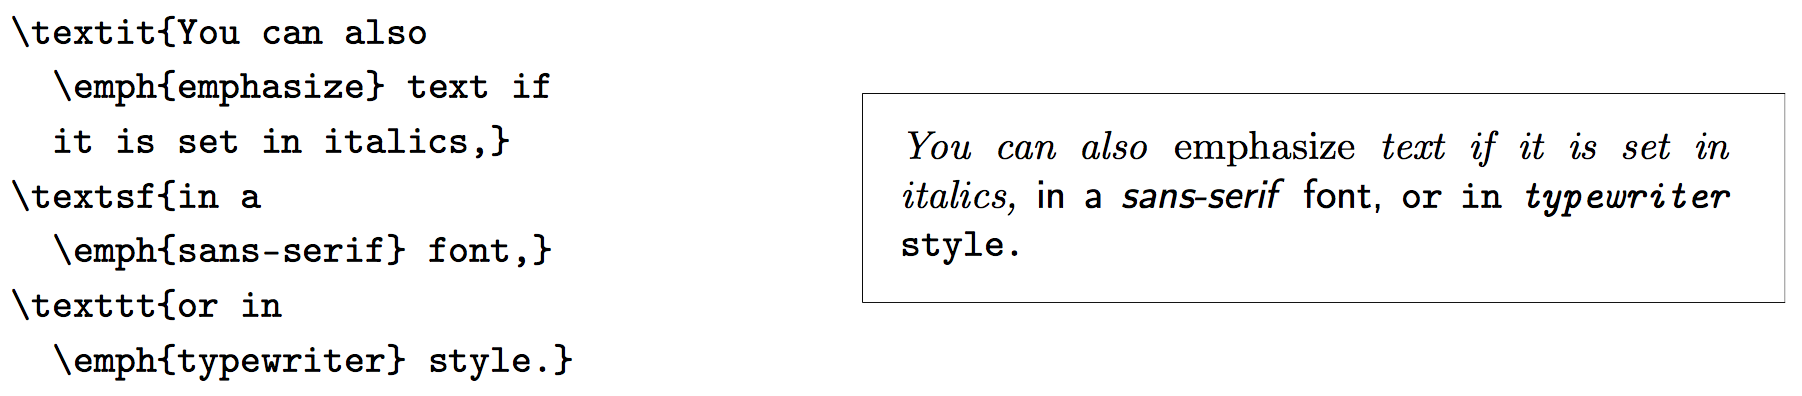
\includegraphics[width=0.6\textwidth]{figures/2_10_emph2}
\end{figure}
\end{frame}


%---------------------------------------------------------------
\begin{frame}{환경}{(example06.tex)}
%---------------------------------------------------------------
\begin{block}{\textbackslash begin\{\emph{environment}\} \ \emph{text} \ \textbackslash end\{\emph{environment}\}}
\begin{itemize}
  \item itemize
  \item enumerate
  \item descriptions
\end{itemize}
\end{block}

\begin{figure}
  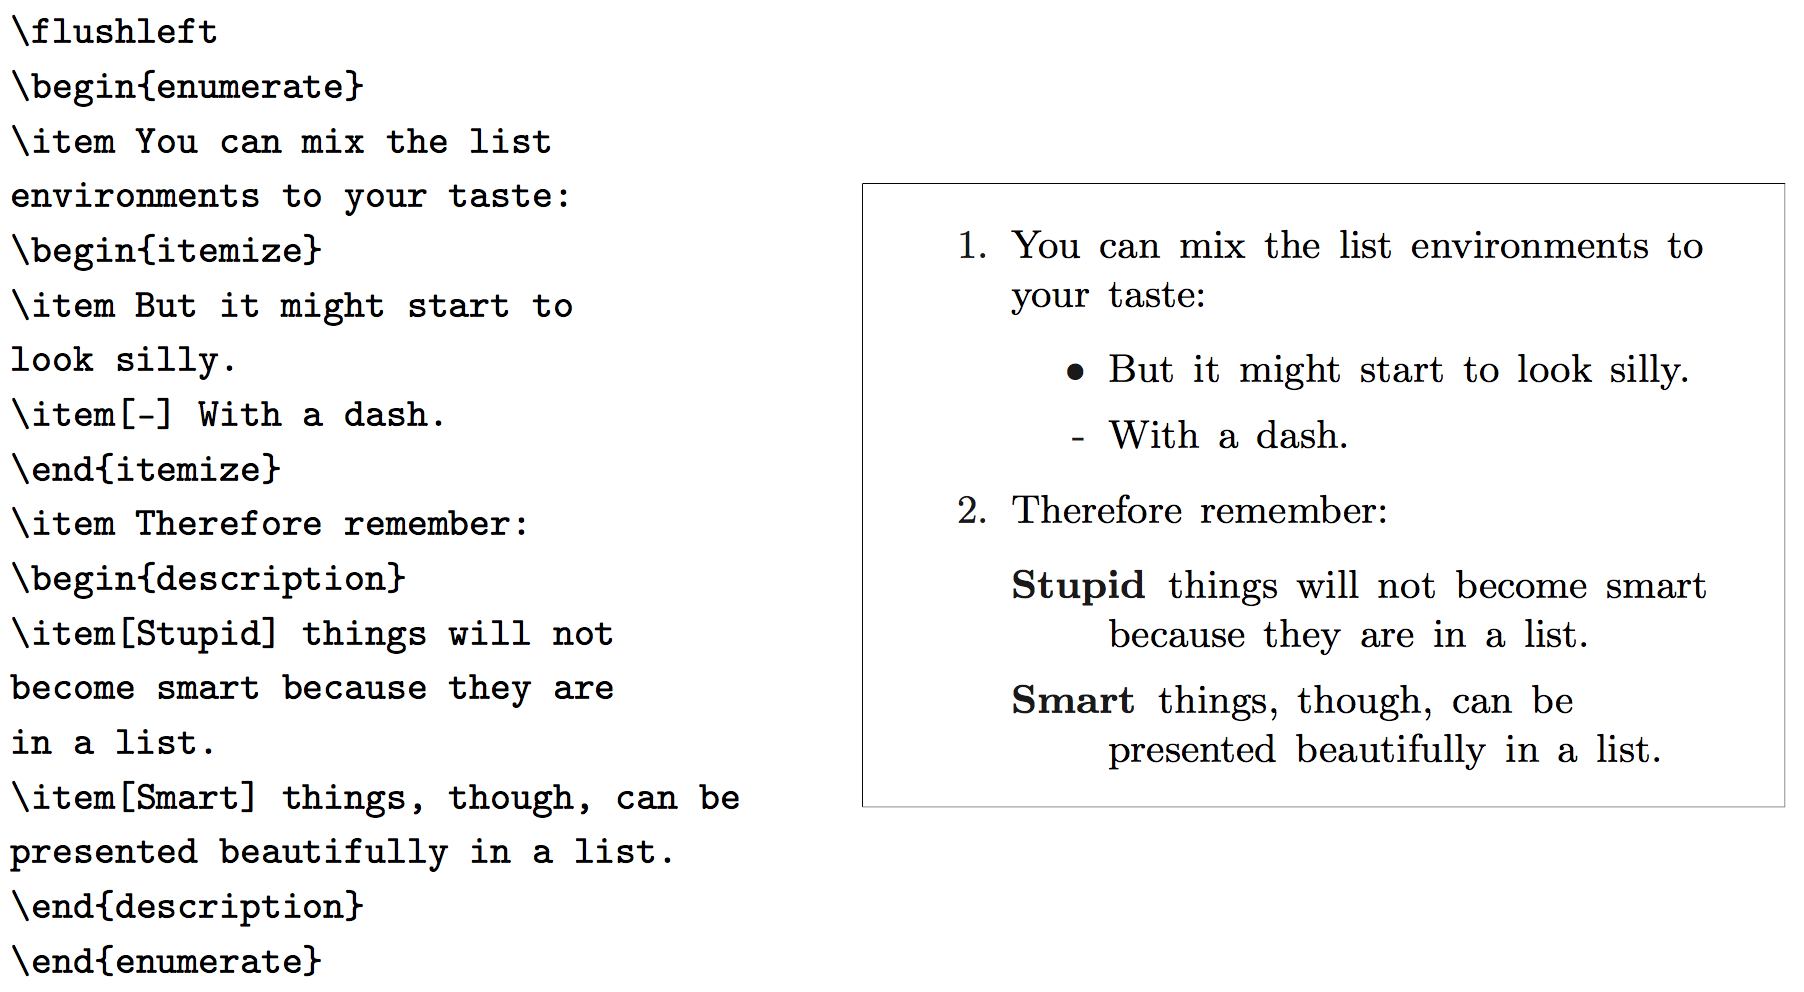
\includegraphics[width=0.5\textwidth]{figures/2_11_1_environment}
\end{figure}
\end{frame}


%---------------------------------------------------------------
\begin{frame}[fragile]{Verbatim 환경}
%---------------------------------------------------------------
\begin{block}{\textbackslash begin\{\emph{verbatim}\} \textbackslash end\{\emph{verbatim}\}}
\begin{itemize}
  \item begin-end 환경
  \begin{itemize}
    \item 텍스트는 마치 타자를 친 것과 같이 \LaTeX{} 명령이 전혀
      수행되지 않고 모든 줄바꿈과 공백이 입력된 그대로 출력된다.
    \item 코드를 직접 삽입할 때 좋다.
  \end{itemize}
  \item \verb|\verb+text+| inline 환경
\end{itemize}
\end{block}

\begin{figure}
  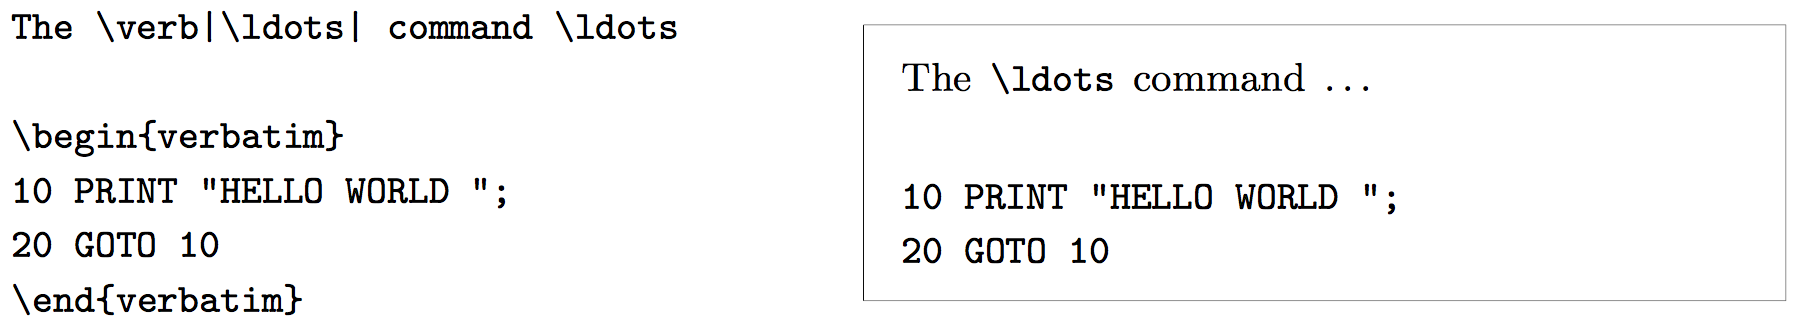
\includegraphics[width=0.7\textwidth]{figures/2_11_5_verbatim}
\end{figure}
\end{frame}


%---------------------------------------------------------------
\begin{frame}[fragile]{Tabular 환경 (1)}{\textbackslash begin\{tabular\}[\emph{pos}]\{\emph{table spec}\}}
%---------------------------------------------------------------
\begin{block}{}
\begin{figure}
  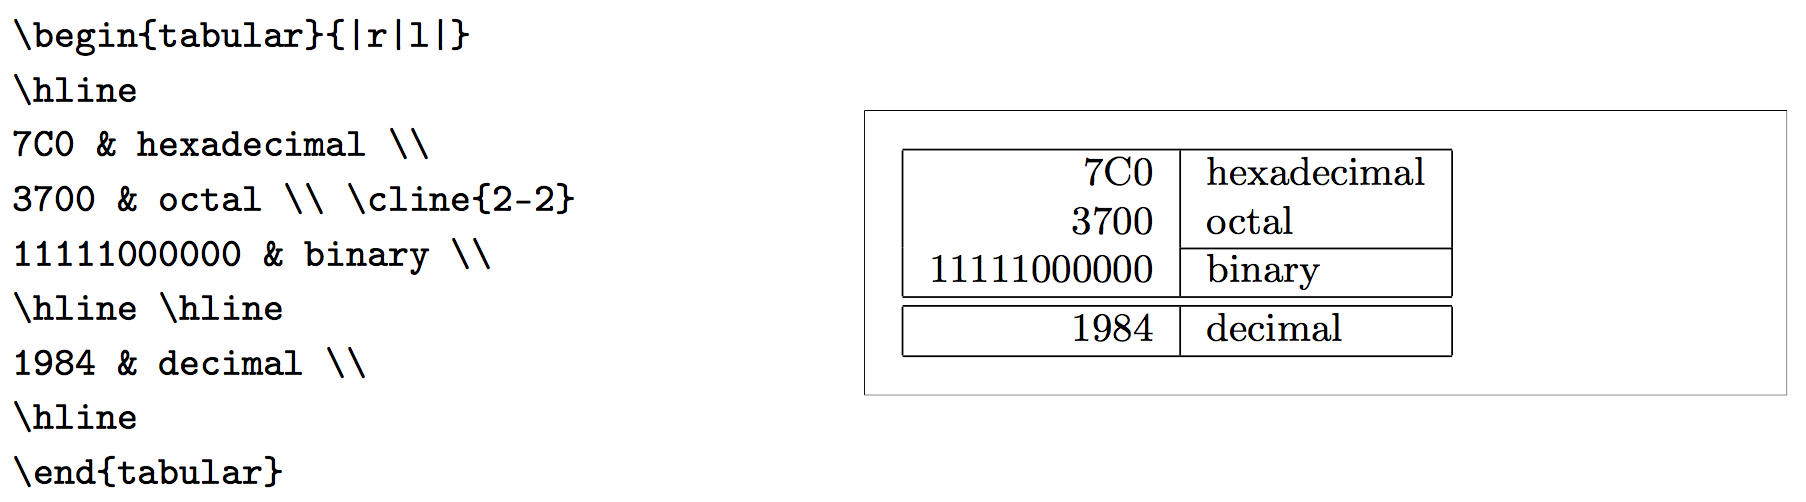
\includegraphics[width=0.7\textwidth]{figures/2_11_6_tabular1}
\end{figure}
\end{block}

\begin{block}{}
\begin{figure}
  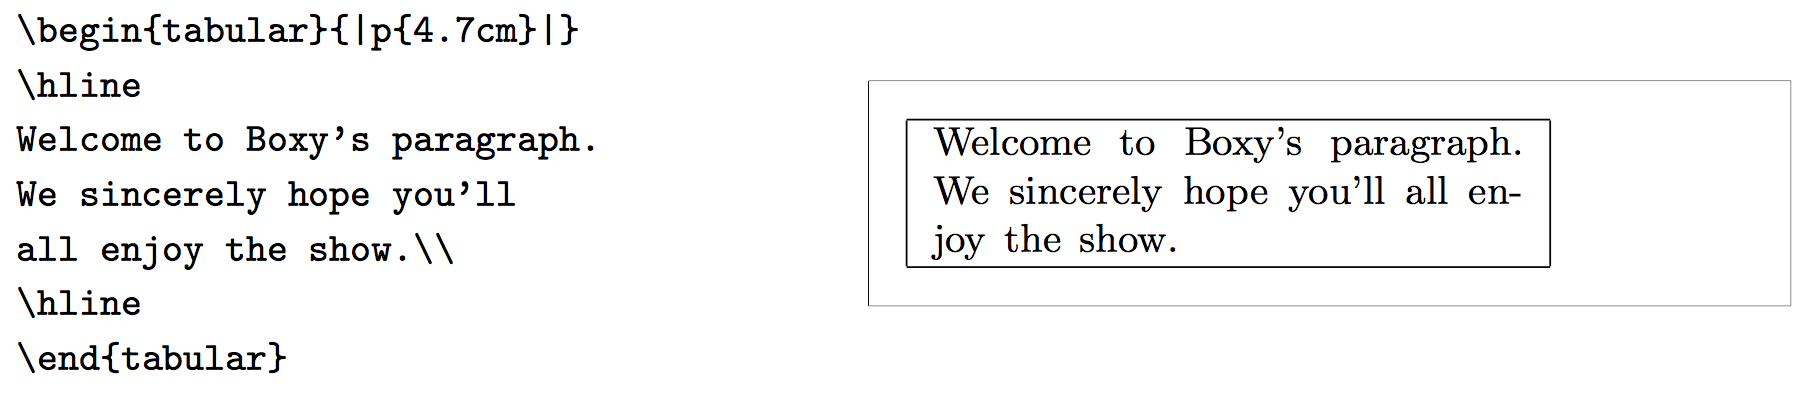
\includegraphics[width=0.7\textwidth]{figures/2_11_6_tabular2}
\end{figure}
\end{block}
\end{frame}


%---------------------------------------------------------------
\begin{frame}{Tabular 환경 (2)}{\textbackslash begin\{tabular\}[\emph{pos}]\{\emph{table spec}\}}
%---------------------------------------------------------------
\begin{block}{}
\begin{figure}
  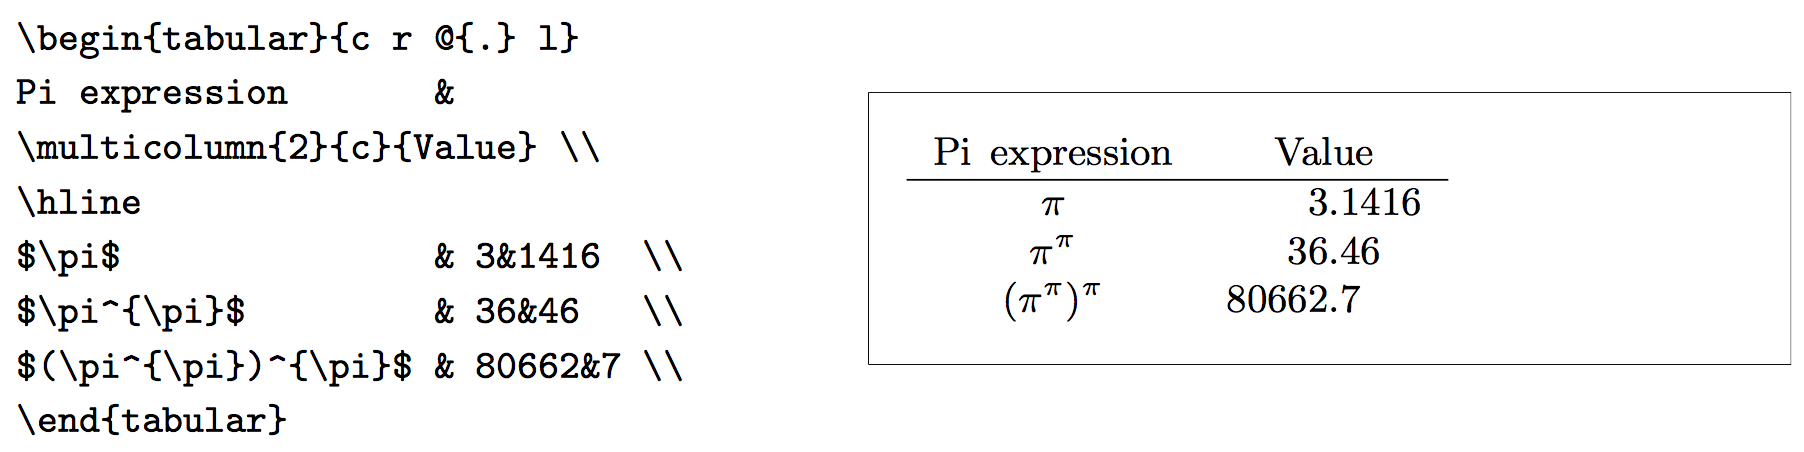
\includegraphics[width=0.7\textwidth]{figures/2_11_6_tabular3}
\end{figure}
\end{block}

\begin{block}{}
\begin{figure}
  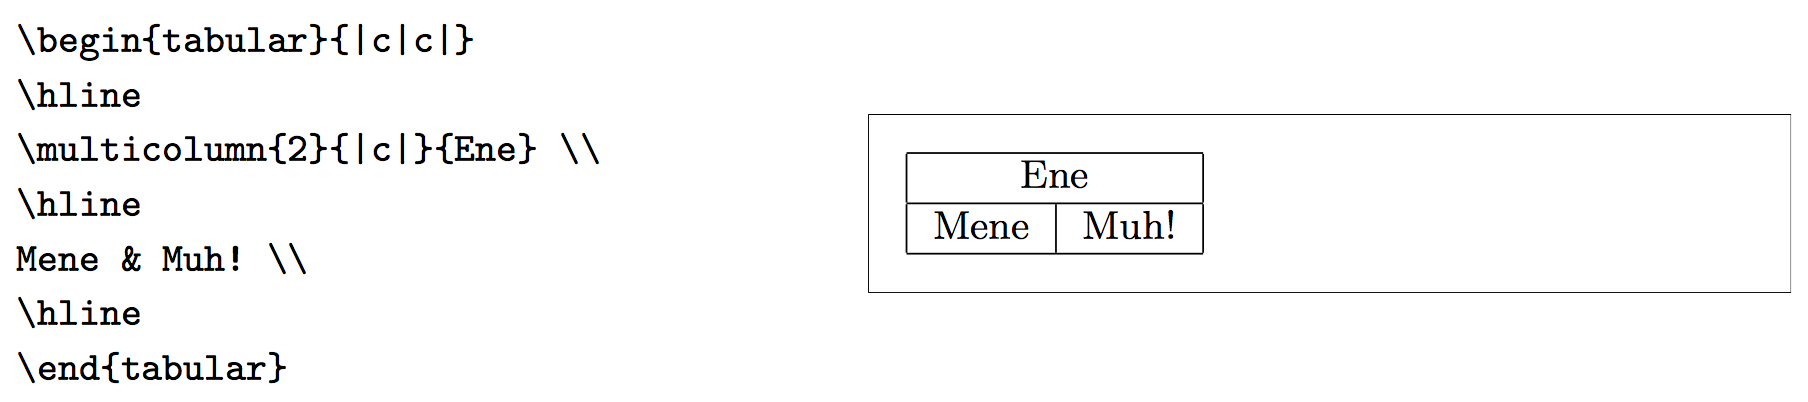
\includegraphics[width=0.7\textwidth]{figures/2_11_6_tabular4}
\end{figure}
\end{block}
\end{frame}


%---------------------------------------------------------------
\begin{frame}{떠다니는 개체 (1)}
%---------------------------------------------------------------
\begin{block}{floating objects}
\begin{itemize}
  \item 그림과 표는 여러 쪽에 걸쳐 나뉠 수 없기 때문에 특별히 다루어야 한다.
  \item 현재 쪽에 들어가지 않는 그림이나 표를 "떠다니게"해서 다음 쪽으로 넘기고 현재 쪽은 본문으로 채운다.
\end{itemize}
\end{block}

\begin{block}{\textbackslash begin\{figure\}[\emph{placement specifier}] or \textbackslash begin\{table\}[\emph{placement specifier}]}
\begin{itemize}
  \item \emph{placement specifier}로 위치를 특정지을 수 있으나 굳이 그렇게 하지 않는 것이 정신건강에 좋다.
  \item \LaTeX이 알아서 위치를 잡아주는 것이 더 자연스럽다.
\end{itemize}
\end{block}
\end{frame}


%---------------------------------------------------------------
\begin{frame}[fragile]{떠다니는 개체 (2)}
%---------------------------------------------------------------
\begin{block}{보통 쓰는 방법}
\begin{lstlisting}
\usepackage{graphicx}

Figure~\ref{white} is an example of Pop-Art.
\begin{figure}[!hbp]
  \includegraphics[width=0.7\textwidth]{figures/some_figure}
  \caption{Five by Five in Centimetres.}
  \label{fig:white}
\end{figure}
\end{lstlisting}

\begin{itemize}
  \item 파일은 보통 vector image를 사용한다.
  \item .eps, .pdf 등을 사용하자.
  \item .jpg, .png 는 사용하지 말자. (어차피 컴파일도 안됨)
\end{itemize}
\end{block}
\end{frame}



%---------------------------------------------------------------
\section{수식 조판하기}
%---------------------------------------------------------------
\begin{frame}{수학식 (1)}
%---------------------------------------------------------------
\begin{block}{}
\begin{itemize}
  \item 수학식은 \emph{inline}으로 조판될 수도 있고
  \item 별도 단락으로 조판될 수도 있다.
\end{itemize}
\end{block}

\begin{block}{inline}
  \textbackslash 와 \textbackslash 사이 또는 \$와 \$사이, 또는 \textbackslash begin\{math\}와 \textbackslash end\{math\} 사이

\begin{figure}
  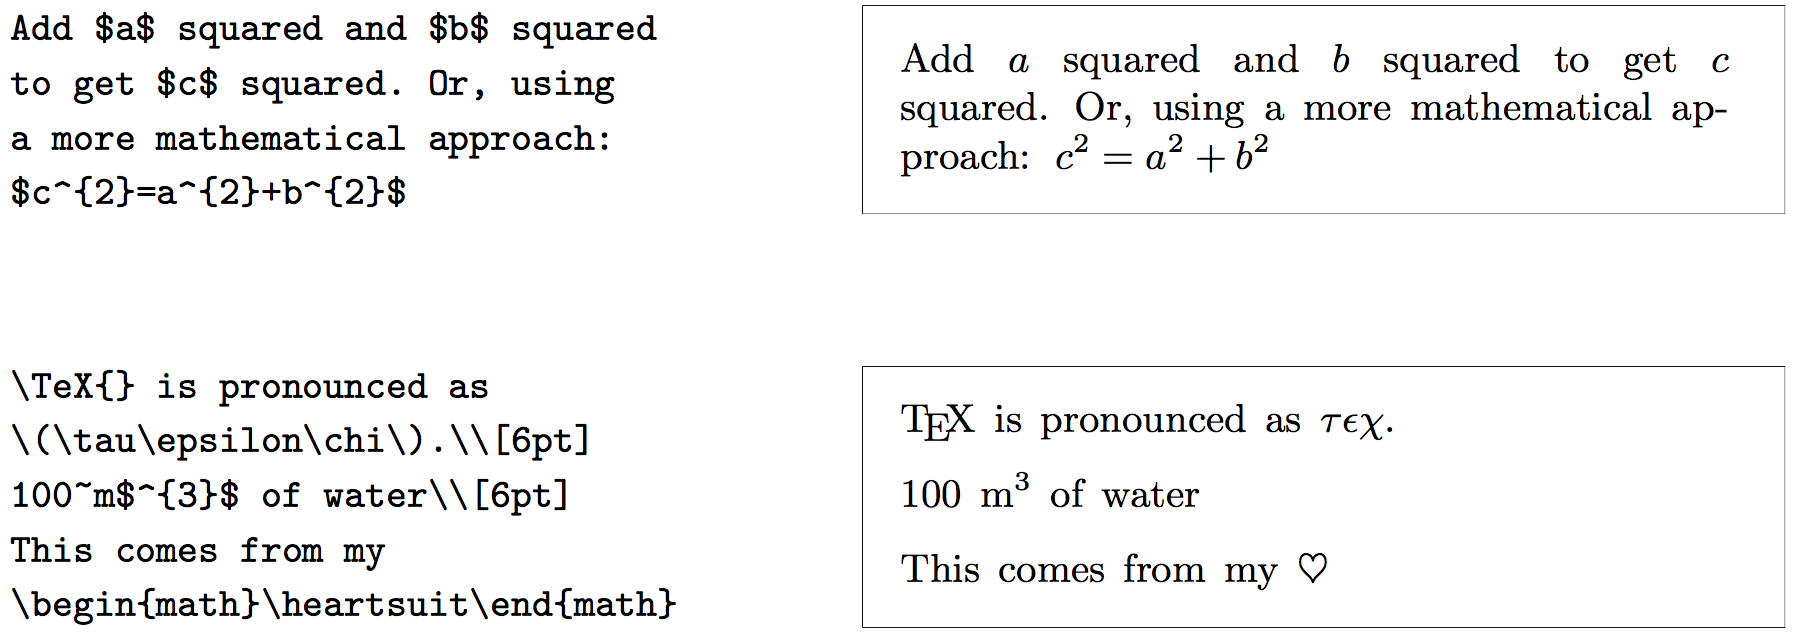
\includegraphics[width=0.7\textwidth]{figures/3_1_1_inline}
\end{figure}
\end{block}

\end{frame}


%---------------------------------------------------------------
\begin{frame}{수학식 (2)}
%---------------------------------------------------------------
\begin{block}{displaymath}
\begin{figure}
  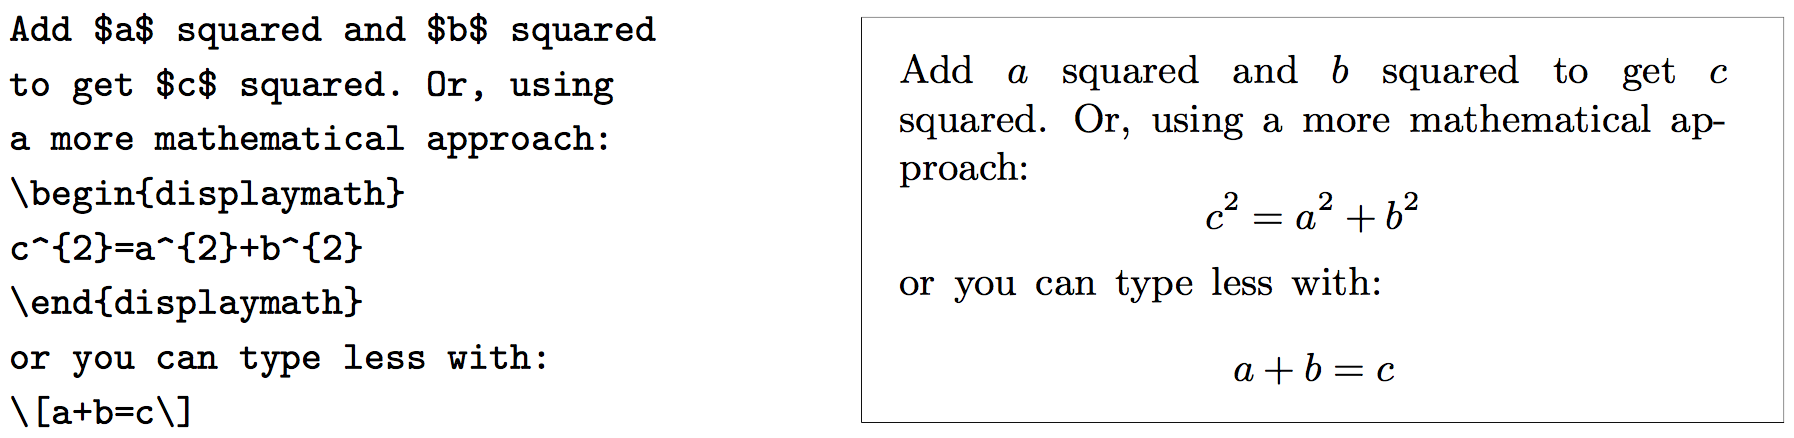
\includegraphics[width=0.7\textwidth]{figures/3_1_2_displaymath}
\end{figure}
\end{block}

\begin{block}{equation}
\begin{figure}
  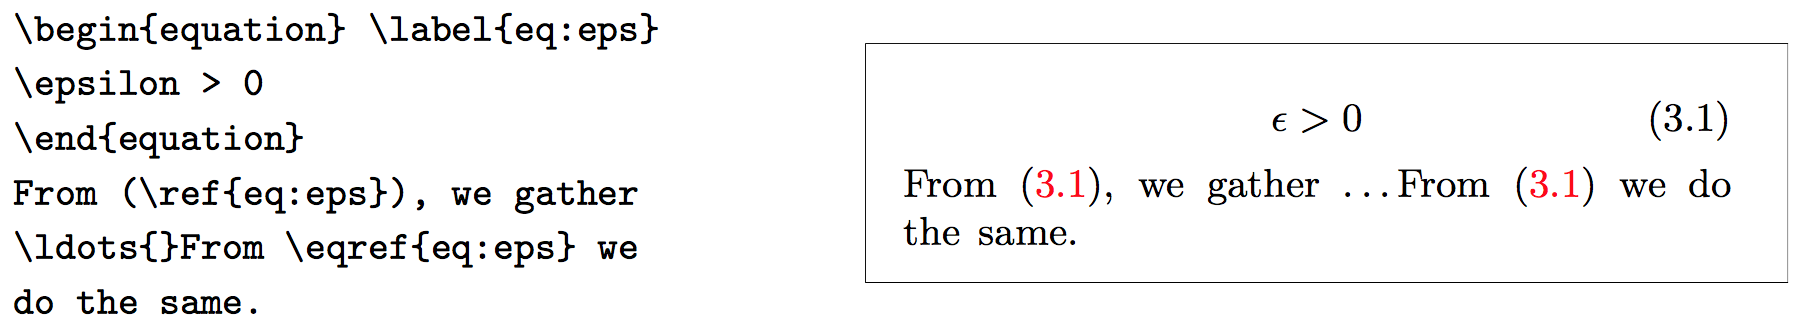
\includegraphics[width=0.7\textwidth]{figures/3_1_3_equation}
\end{figure}
\end{block}
\end{frame}


%---------------------------------------------------------------
\begin{frame}{수학 모드}
%---------------------------------------------------------------
\begin{block}{수학 모드의 특징}
\begin{enumerate}
  \item 빈칸과 줄바꿈은 아무런 의미도 없다. 수식의 공백은 수학식 표현의 논리에 따라 정해지며 이것을 제어하려면 \textbackslash, 또는 \textbackslash quad 또는 \textbackslash qquad와 같은 특별한 명령으로 지정해야 한다.
  \item 빈줄은 허용되지 않는다. 하나의 수식을 여러문단으로 적을 수 없다.
  \begin{itemize}
    \item \textbackslash begin\{array\} 같은 환경을 쓰면 해결할 수 있다.
  \end{itemize}
  \item 각 글자는 변수명으로 간주되어 변수로 조판될 것이다. 일반 텍스트(정상적인 곧게 선 글꼴과 일반적인 간격)를 수식 안에서 조판하고자 한다면 텍스트를 \textbackslash textrm\{...\} 명령 안에 넣어야 한다.
\end{enumerate}
\end{block}

\begin{figure}
  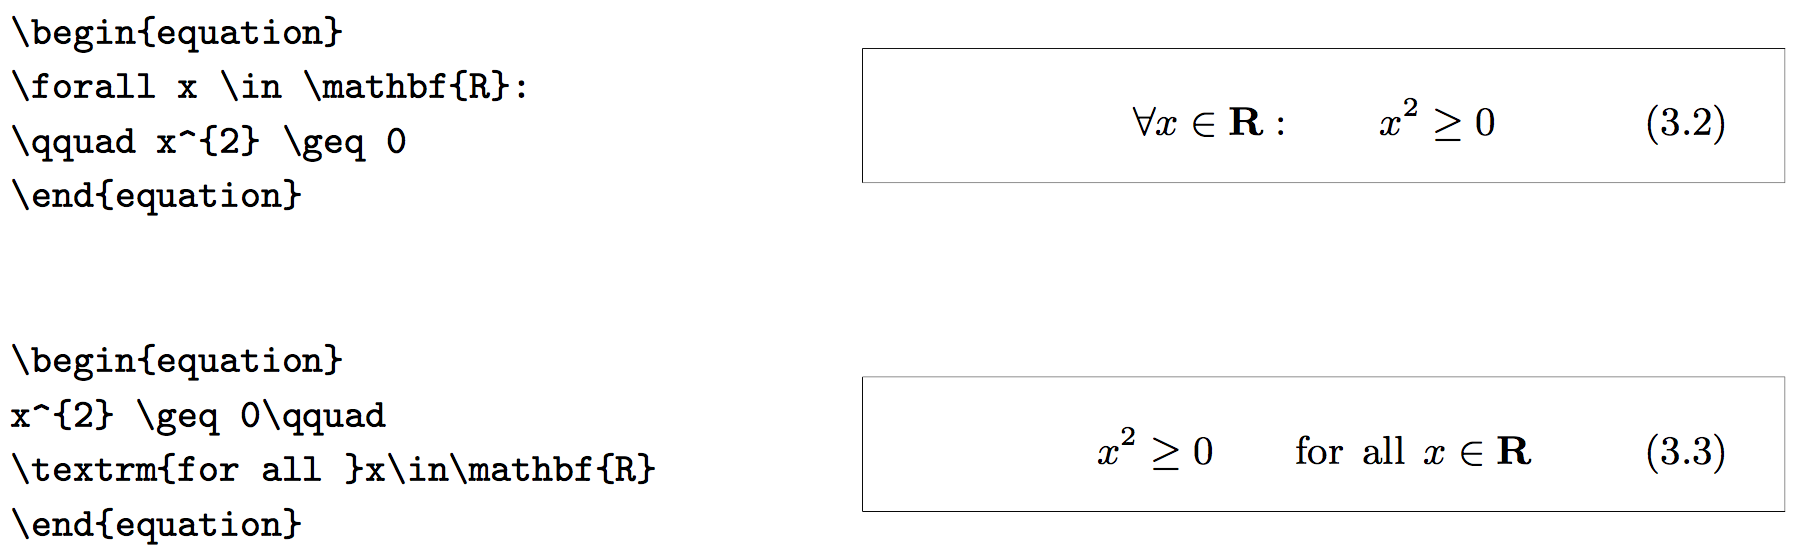
\includegraphics[width=0.7\textwidth]{figures/3_1_4_math_mode}
\end{figure}
\end{frame}


%---------------------------------------------------------------
\begin{frame}{수학 모드에서 묶기}
%---------------------------------------------------------------
\begin{block}{중괄호를 써서 묶는다}
\begin{figure}
  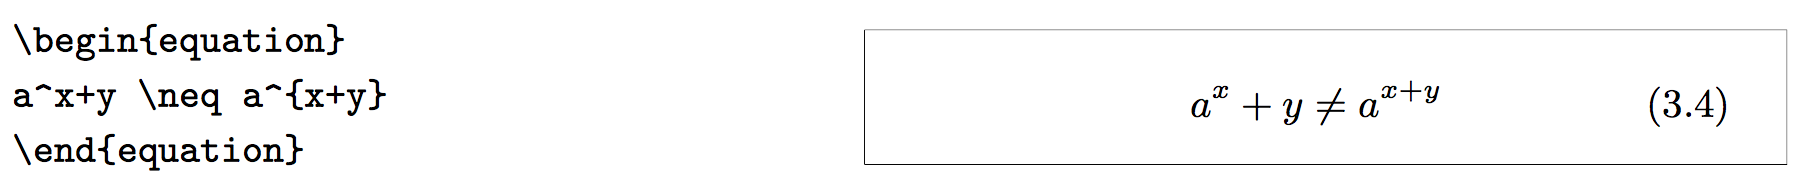
\includegraphics[width=0.7\textwidth]{figures/3_2_binding}
\end{figure}
\end{block}
\end{frame}


%---------------------------------------------------------------
\begin{frame}{수식 구성하기 (1)}
%---------------------------------------------------------------
\begin{block}{그리스 문자}
\begin{figure}
  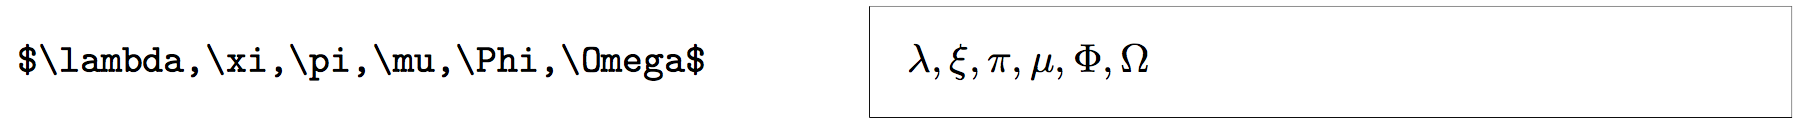
\includegraphics[width=0.7\textwidth]{figures/3_3_1_greek}
\end{figure}
\end{block}

\begin{block}{위첨자, 아랫첨자}
\begin{figure}
  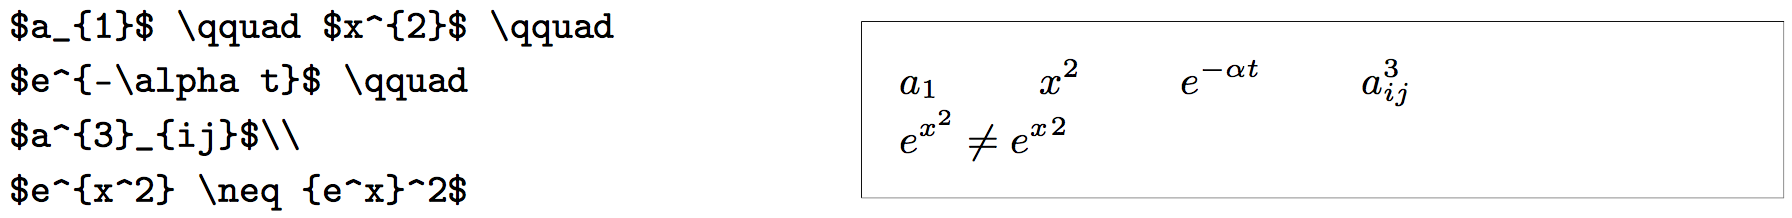
\includegraphics[width=0.7\textwidth]{figures/3_3_2_script}
\end{figure}
\end{block}

\begin{block}{제곱근}
\begin{figure}
  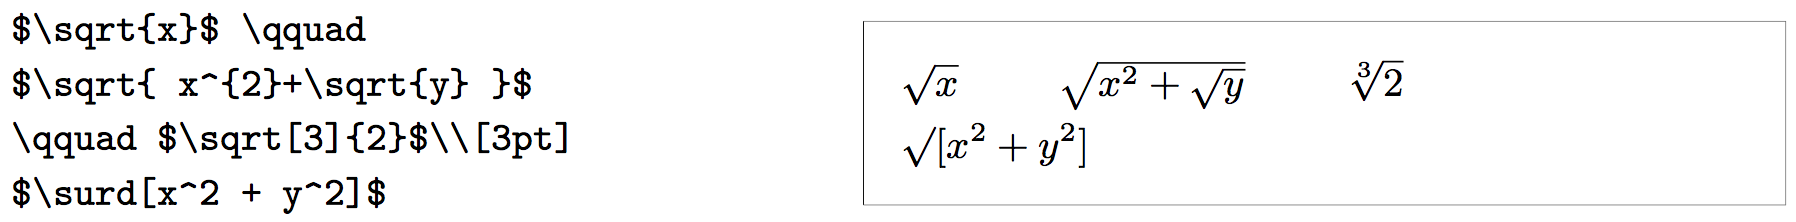
\includegraphics[width=0.7\textwidth]{figures/3_3_3_sqrt}
\end{figure}
\end{block}
\end{frame}


%---------------------------------------------------------------
\begin{frame}{수식 구성하기 (2)}
%---------------------------------------------------------------
\begin{block}{overline and underline}
\begin{figure}
  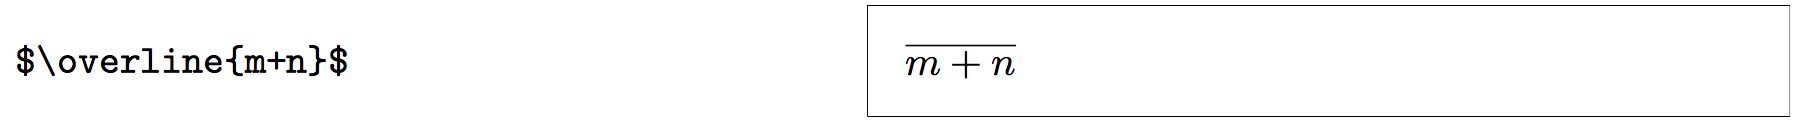
\includegraphics[width=0.7\textwidth]{figures/3_3_4_underline}
\end{figure}
\end{block}

\begin{block}{overbrace and underbrace}
\begin{figure}
  
\includegraphics[width=0.7\textwidth]{figures/3_3_5_underbrace}
\end{figure}
\end{block}

\begin{block}{미분 표시}
\begin{figure}
  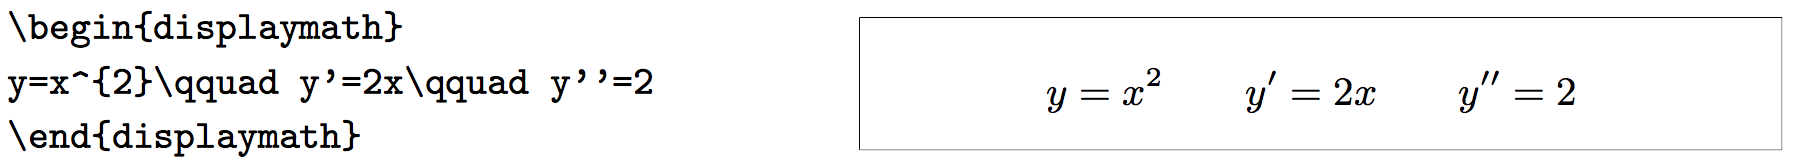
\includegraphics[width=0.7\textwidth]{figures/3_3_6_derivative}
\end{figure}
\end{block}
\end{frame}


%---------------------------------------------------------------
\begin{frame}{수식 구성하기 (3)}
%---------------------------------------------------------------
\begin{block}{dot product}
\begin{figure}
  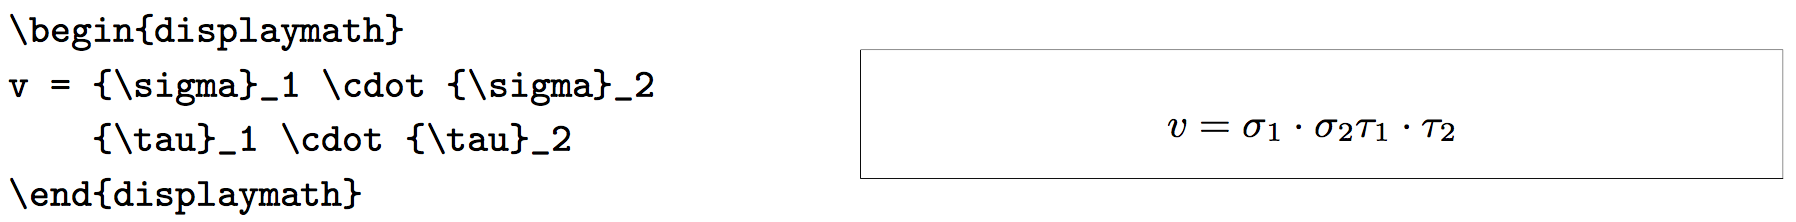
\includegraphics[width=0.7\textwidth]{figures/3_3_7_dot_product}
\end{figure}
\end{block}

\begin{block}{자주쓰는 함수류}
\begin{figure}
  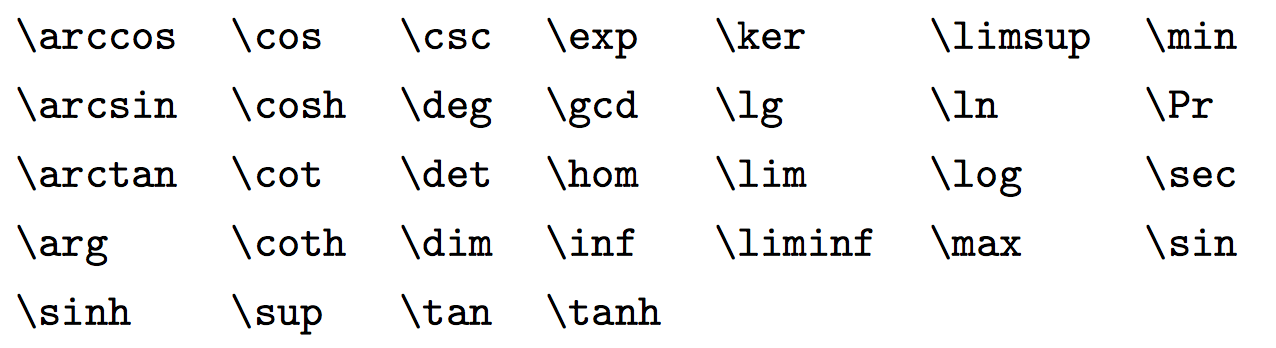
\includegraphics[width=0.7\textwidth]{figures/3_3_8_log}
\end{figure}
\end{block}
\end{frame}


%---------------------------------------------------------------
\begin{frame}{수식 구성하기 (4)}
%---------------------------------------------------------------
\begin{block}{분수 표시}
\begin{figure}
  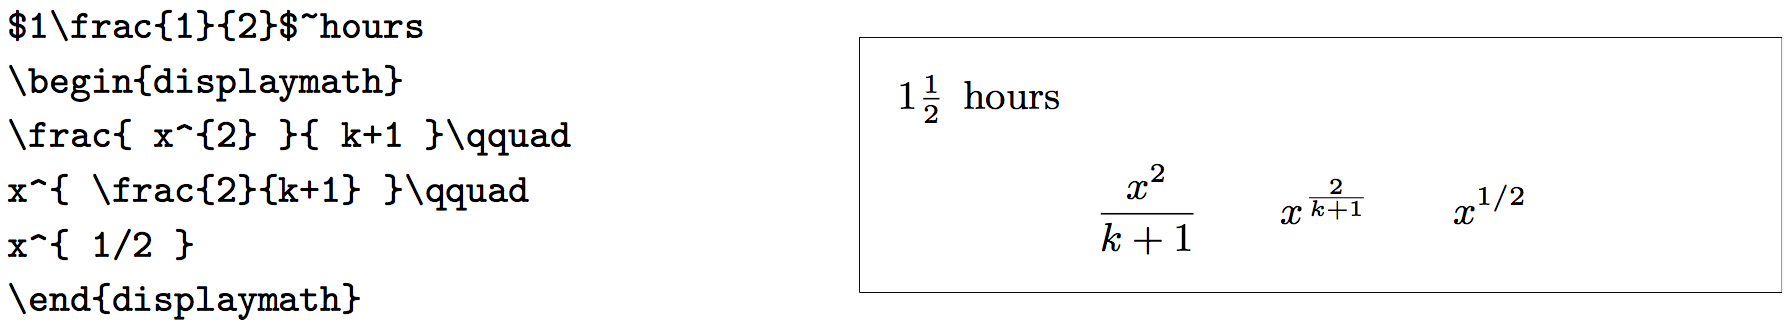
\includegraphics[width=0.7\textwidth]{figures/3_3_9_frac}
\end{figure}
\end{block}

\begin{block}{summation, integral, and production}
\begin{figure}
  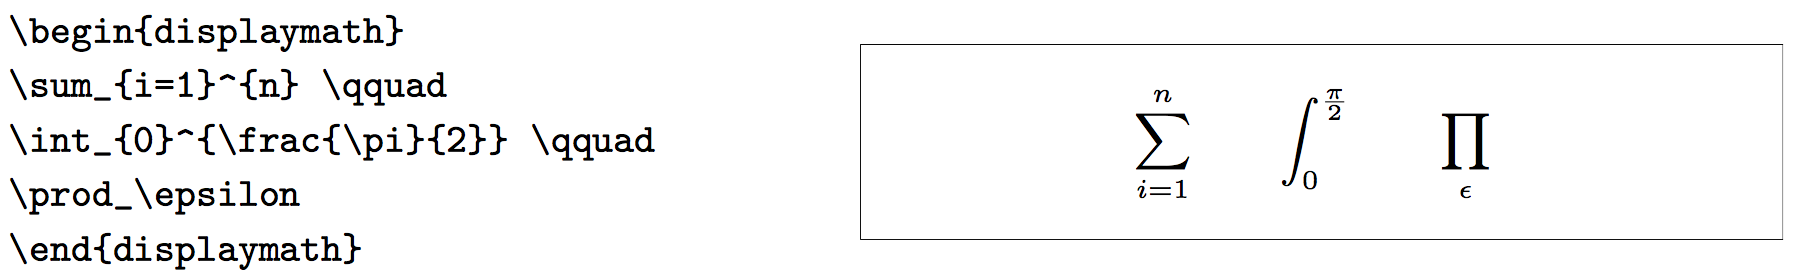
\includegraphics[width=0.7\textwidth]{figures/3_3_10_sum_prod}
\end{figure}
\end{block}
\end{frame}


%---------------------------------------------------------------
\begin{frame}{수식 구성하기 (5)}
%---------------------------------------------------------------
\begin{block}{괄호}
\begin{figure}
  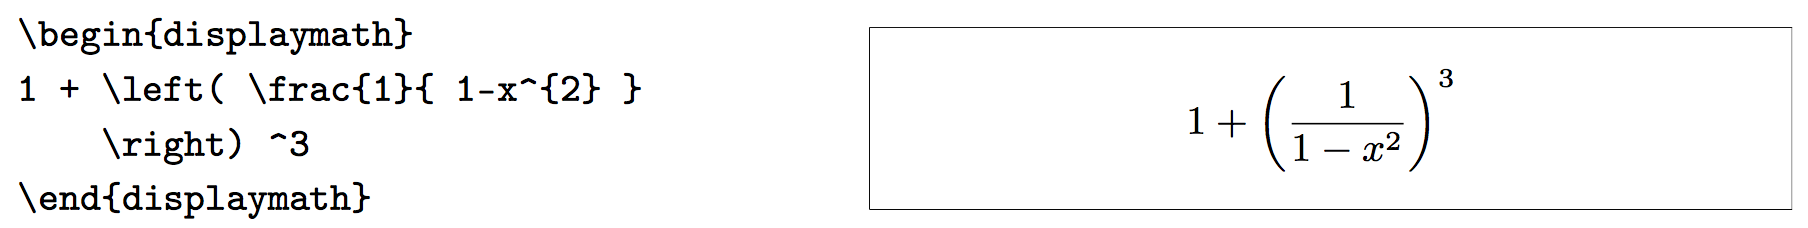
\includegraphics[width=0.7\textwidth]{figures/3_3_11_bracket}\\
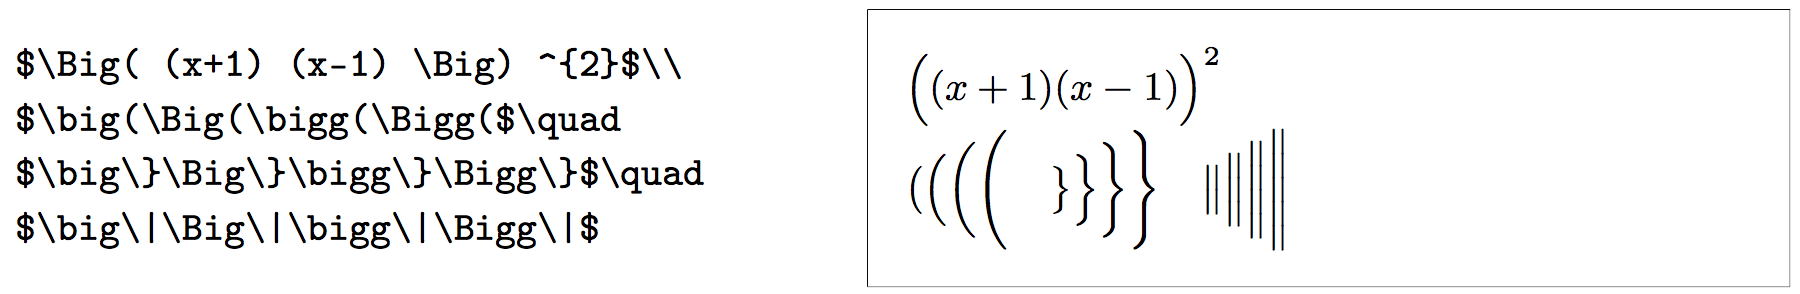
\includegraphics[width=0.7\textwidth]{figures/3_3_12_big_bracket}
\end{figure}

\begin{itemize}
  \item 괄호([], \{\}, ())들에 짝맞춤을 해주면 크기를 적당하게 자동으로 맞춰준다.
  \item 짝맞춤 기호: \textbackslash left, \textbackslash right
  \item \textbackslash left를 쓰면 반드시 \textbackslash right로 닫아준다.
  \item 오른쪽에 닫지 않으려면 '\textbackslash right.' 을 쓰면 된다. 
  \item \textbackslash big,
        \textbackslash Big,
        \textbackslash bigg,
        \textbackslash Bigg 명령으로 직접 크기를 정할수 있다.
\end{itemize}
\end{block}
\end{frame}


%---------------------------------------------------------------
\begin{frame}{수식의 간격}
%---------------------------------------------------------------
\begin{columns}
\begin{column}{0.32\textwidth}
\begin{block}{괄호}
\begin{description}
  \item[\textbackslash ,] 3/18 quad
  \item[\textbackslash :] 4/18 quad
  \item[\textbackslash ;] 5/18 quad
  \item[\textbackslash (space)] 1/2 quad (반각)
  \item[\textbackslash quad] quad (전각)
  \item[\textbackslash qquad] 2 quad (2배각)
\end{description}
\end{block}
\end{column}

\begin{column}{0.6\textwidth}
\begin{figure}
  %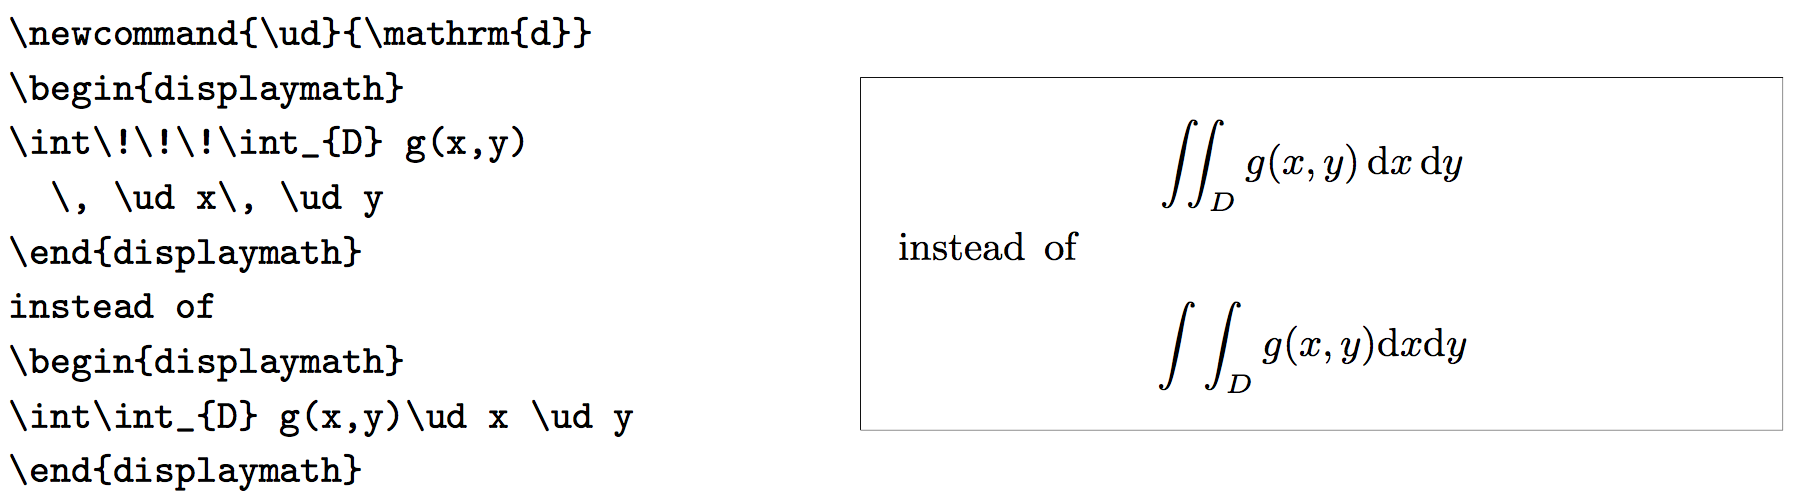
\includegraphics[width=0.6\textwidth]{figures/3_4_quad}
  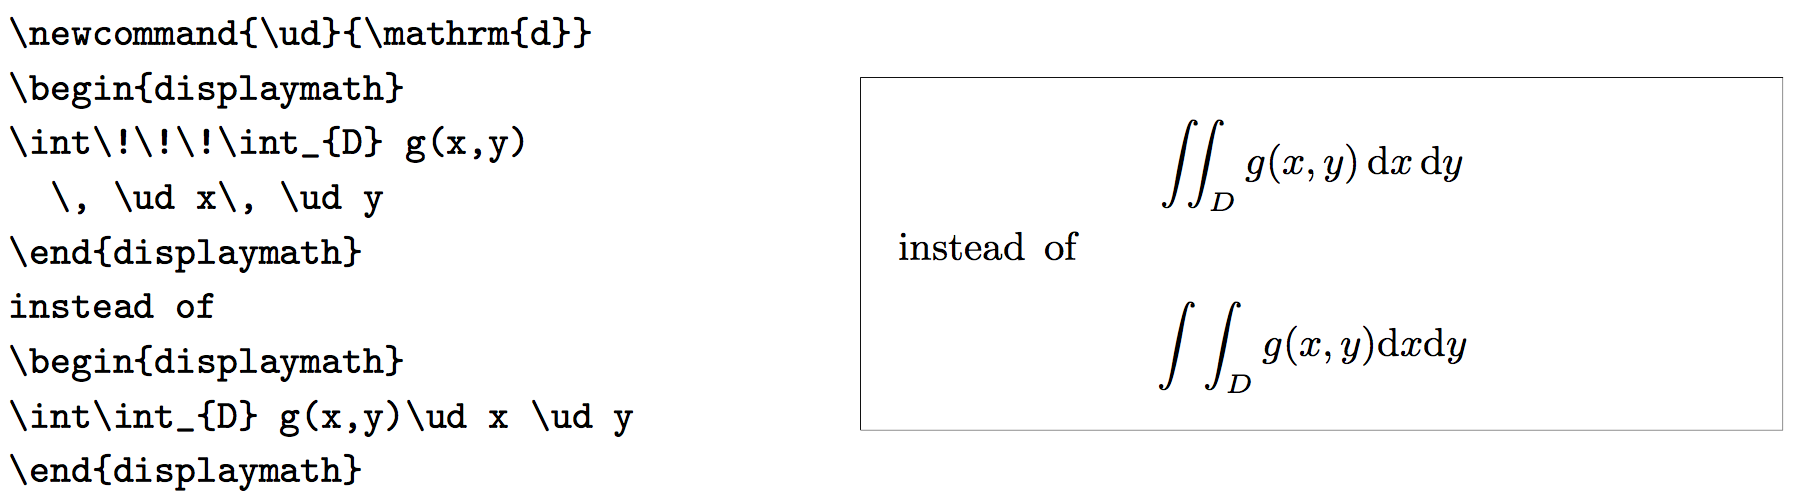
\includegraphics[width=\textwidth]{figures/3_4_quad}
\end{figure}
\end{column}
\end{columns}

\vspace{3ex}
미분의 'd'는 보통 곧은 글꼴로 조판된다는 것에 주의하자.

\end{frame}


%---------------------------------------------------------------
\begin{frame}{세로 줄맞춤이 필요한 요소들 (1)}
%---------------------------------------------------------------
\begin{block}{행렬 조판}
\begin{itemize}
  \item array 환경을 쓴다. tabular 환경과 비슷하다.
\end{itemize}

\begin{figure}
  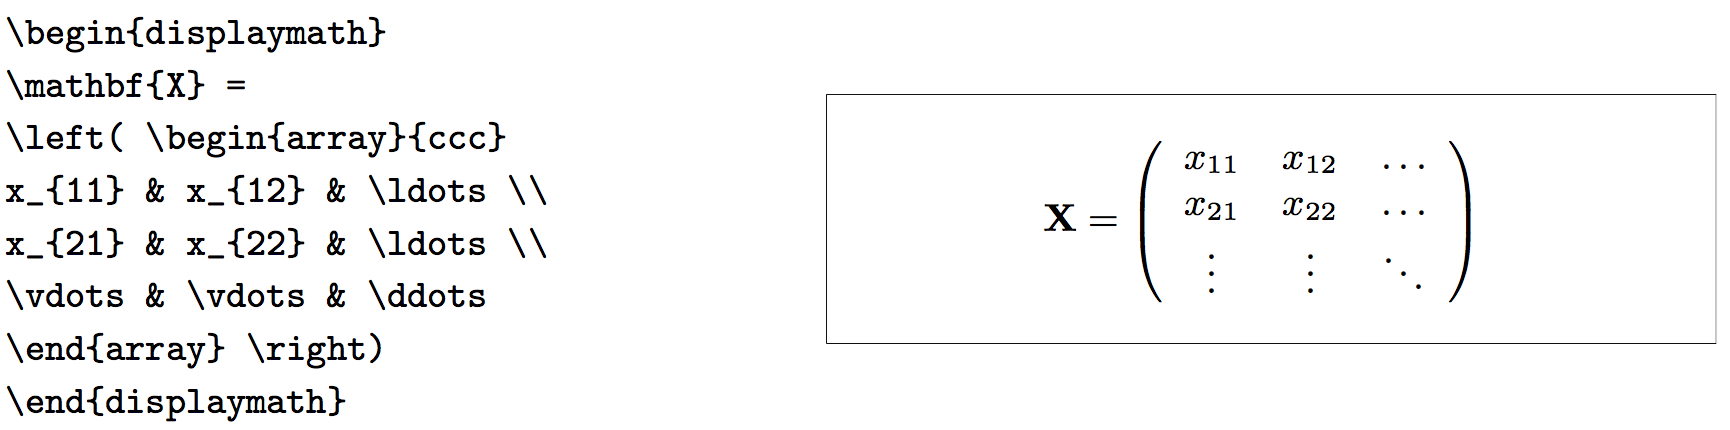
\includegraphics[width=0.7\textwidth]{figures/3_5_1_matrix}\\
  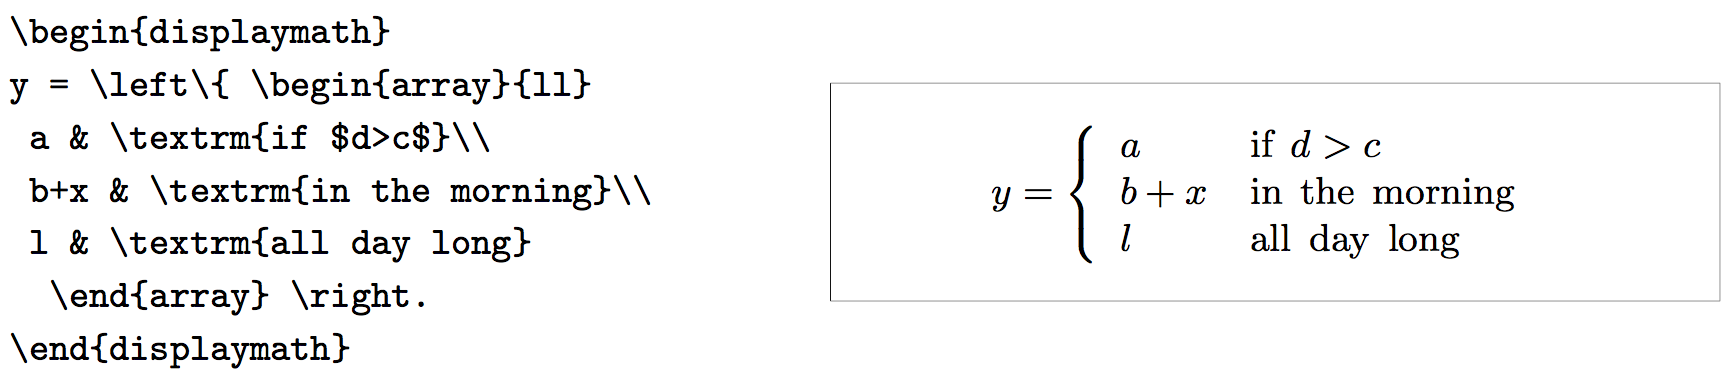
\includegraphics[width=0.7\textwidth]{figures/3_5_2_matrix}
\end{figure}
\end{block}
\end{frame}



%---------------------------------------------------------------
\begin{frame}{세로 줄맞춤이 필요한 요소들 (2)}
%---------------------------------------------------------------
\begin{block}{긴 수식}
\begin{figure}
  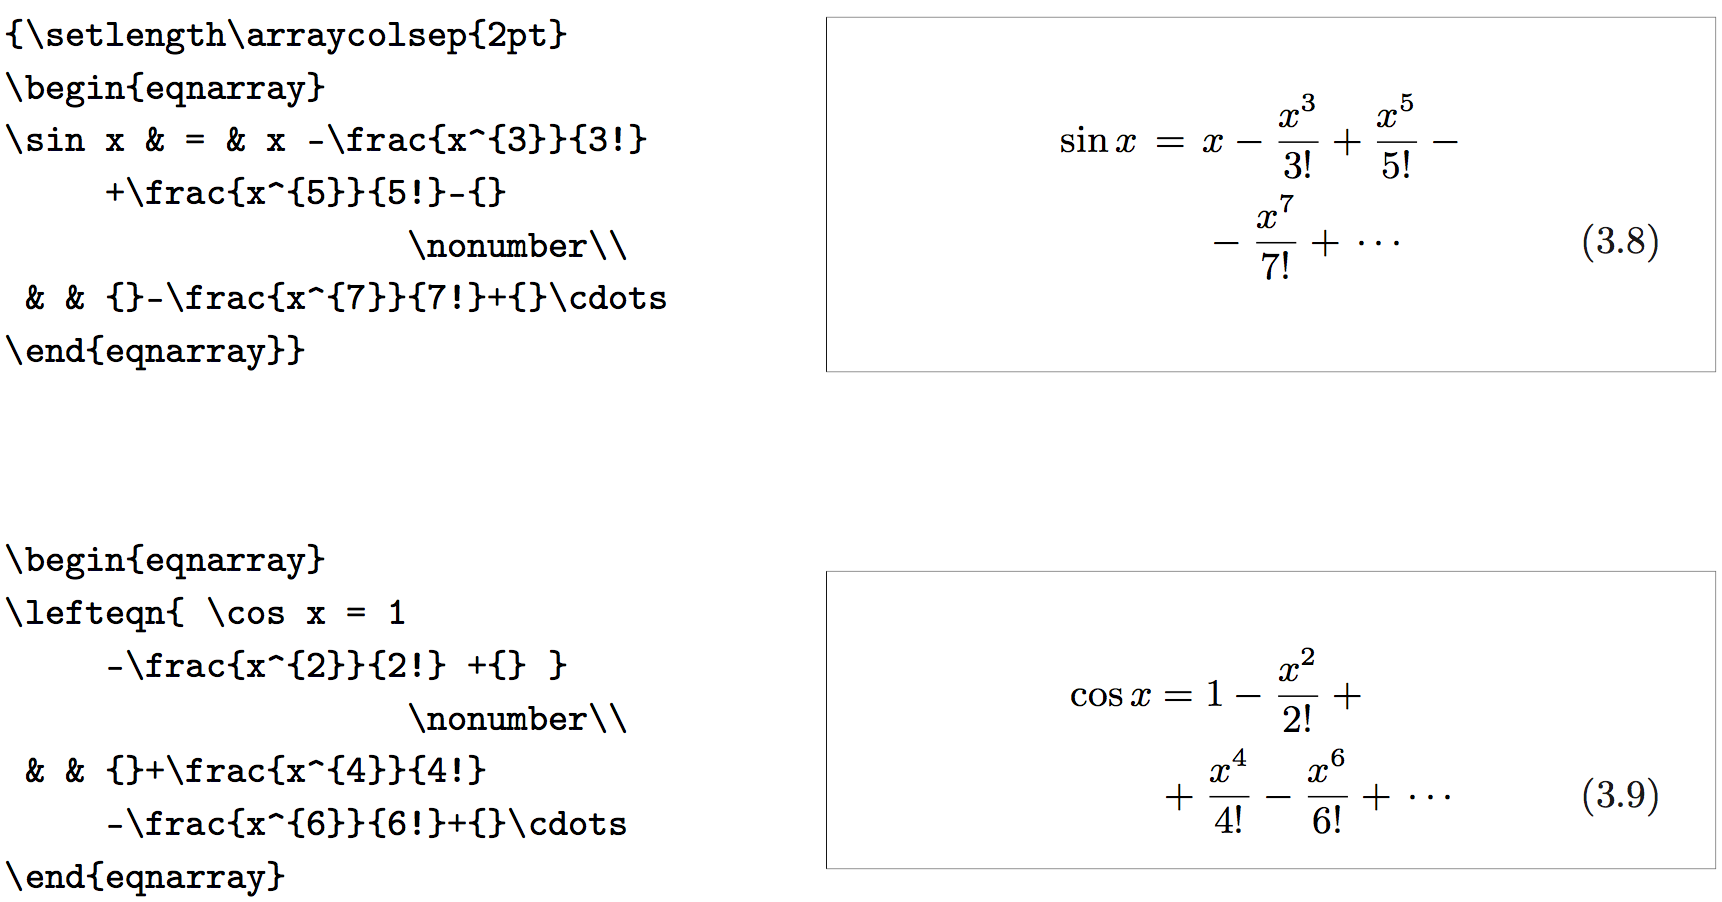
\includegraphics[width=0.7\textwidth]{figures/3_5_3_long_equation}
\end{figure}
\end{block}
\end{frame}


%---------------------------------------------------------------
\begin{frame}{수학 볼드 기호}
%---------------------------------------------------------------
\begin{block}{벡터를 표현할 때 주로 쓴다 (\textbackslash boldsymbol)}
\begin{figure}
  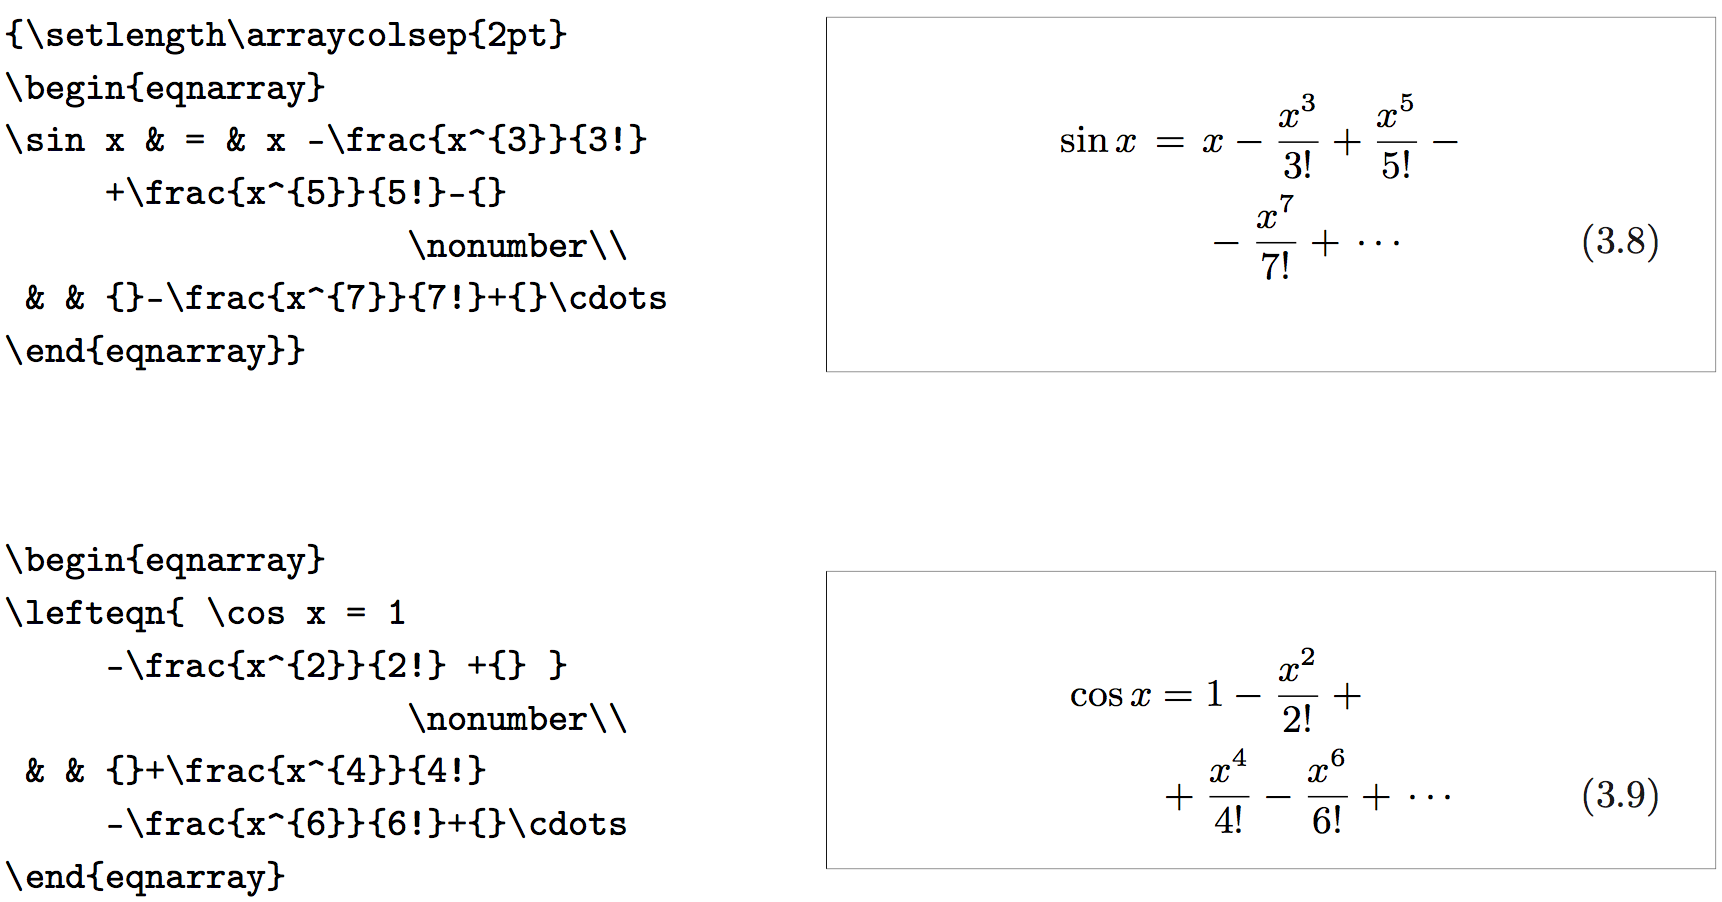
\includegraphics[width=0.7\textwidth]{figures/3_5_3_long_equation}
\end{figure}
\end{block}
\end{frame}


%---------------------------------------------------------------
\begin{frame}{수학 기호 일람 (1)}
%---------------------------------------------------------------
\begin{block}{특정 기호를 사용하려면 여러 패키지들을 써야한다}
\begin{itemize}
  \item amsmath
  \item amssymb
  \item amsthm
  \item amsfonts
  \item 등등
  \item 구글에 latex math symbols 라고 쳐보자
\end{itemize}
\end{block}
\end{frame}


%---------------------------------------------------------------
\begin{frame}{수학 기호 일람 (2)}
%---------------------------------------------------------------
\begin{block}{mathfonts}
\begin{figure}
  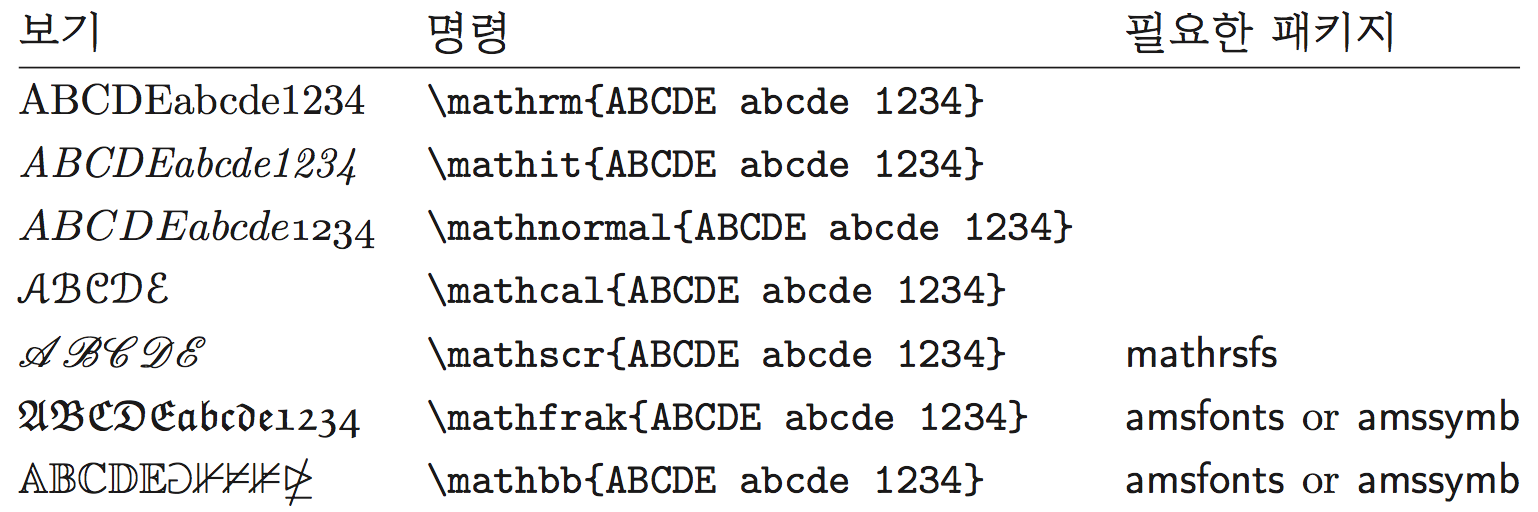
\includegraphics[width=0.7\textwidth]{figures/3_10_math_fonts}
\end{figure}
\end{block}
\end{frame}



%---------------------------------------------------------------
\section{특별한 기능}
%---------------------------------------------------------------
\begin{frame}{참고문헌}
%---------------------------------------------------------------
\begin{block}{example07.tex}
\begin{itemize}
  \item .bib 파일을 만든다.
  \begin{itemize}
    \item Mendeley, Papers 같은 프로그램을 이용하면 된다.
  \end{itemize}
  \item latex $\rightarrow$ bibtex $\rightarrow$ latex $\rightarrow$ latex 순서로 컴파일 한다.
\end{itemize}
\end{block}
\end{frame}


%---------------------------------------------------------------
\begin{frame}[fragile]{beamer}
%---------------------------------------------------------------
\begin{block}{자주 쓰는 것들}
\begin{itemize}
  \item 슬라이드 구성
  \begin{itemize}
    \item \verb+\begin{frame}{frametitle} ... \end{frame}+
  \end{itemize}
  \item itemize, enumerate, descriptions
  \item block
  \item vspace\{0.5ex\}
  \item pause
  \item listings: verbatim의 역할
  \item columns
\end{itemize}
\end{block}
\end{frame}









%---------------------------------------------------------------
%\begin{frame}[plain,noframenumbering]
\begin{frame}
%---------------------------------------------------------------
    \center
    \LARGE
    \Rcolor{Thank you for your attention!}
\end{frame}


\end{document}


